\documentclass[12pt,a4paper]{article}

% ---------- Packages ----------
\usepackage[T1]{fontenc}
\usepackage[utf8]{inputenc}
\usepackage{mathptmx}
\usepackage[margin=2.5cm]{geometry}
\usepackage{graphicx}
\graphicspath{{figs/}}
\usepackage{amsmath,amssymb}
\usepackage{siunitx}
\usepackage{booktabs}
\usepackage{caption}
\usepackage[hidelinks]{hyperref}
\usepackage{fancyhdr}
\usepackage{xcolor}
\usepackage{setspace}
\usepackage{enumitem}
\usepackage[nottoc]{tocbibind}
\usepackage{siunitx} % For \SI{val}{unit} formatting
\usepackage{cite}    % For \cite{} handling
\usepackage{circuitikz} 
\usepackage{subcaption}
\usepackage{float}
\usepackage{tikz}
\usepackage{pgfplots}
\usepackage{caption}
\pgfplotsset{compat=1.18}


\hypersetup{pdftitle={TMR Sensor Final Year Technical Report}, pdfauthor={Sam Ye}}

\newcommand{\todo}[1]{\textcolor{red}{\textbf{[TODO: #1]}}}

\pagestyle{fancy}
\fancyhf{}
\fancyfoot[C]{\thepage}
\renewcommand{\headrulewidth}{0pt}

\setlength{\parskip}{0.4em}
\setlength{\parindent}{0pt}

\begin{document}

% ============================================================
% TITLE PAGE (excluded from page count)
% ============================================================
\begin{titlepage}
\centering
\vspace*{1.5cm}
{\large Department of Electrical, Computer, and Software Engineering \\ The University of Auckland \par}
\vspace{2.5cm}
{\Huge\bfseries Characterisation, Field Modelling, and Radiation Testing of a Commercial Tunnelling Magnetoresistance (TMR) Sensor for CubeSat Attitude Determination and Control \par}
\vspace{2cm}
{\Large Final Year Technical Report \par}
\vspace{2.5cm}
{\large\bfseries Sam Ye \par}
\vspace{0.6cm}
{\large Supervisor: Dariusz Kacprzak \par}
\vspace{0.2cm}
{\large Project Partner: Daniel Tieu \par}
\vfill
{\large \todo{insert submission date} \par}
\end{titlepage}


\clearpage
\section*{Acknowledgements}
\addcontentsline{toc}{section}{Acknowledgements}

The author thanks project supervisor Dariusz Kacprzak for guidance throughout this project, and project partner Daniel Tieu for his work on the parallel thermal-cycling test campaign. \todo{Add any further acknowledgements -- e.g.\ workshop/lab staff, the radiation-testing facility or operator, or funding sources -- once confirmed.}

Nitish, Aaron, Arnesh, Alex, jensen, Uzayr

fix formatting number an TOC

\clearpage

% ============================================================
% ABSTRACT (excluded from page count)
% ============================================================
\pagenumbering{roman}
\setcounter{page}{2}
\section*{Abstract}
\addcontentsline{toc}{section}{Abstract}

Tunnelling magnetoresistance (TMR) sensors offer chip-scale, high-sensitivity magnetic field detection that is attractive for CubeSat Attitude Determination and Control System (ADCS) and Electrical Power System (EPS) applications, yet the technology remains at a low Technology Readiness Level (TRL~3) with limited published space-qualification data. This report documents the design, construction, and testing of two custom PCBs built around a commercial-off-the-shelf (COTS) CT100 TMR sensor: a primary board exposing the raw sensor bridge, and an integrated telemetry board adding STM32-based automated logging and an independent current-sense field reference. The CT100's Wheatstone-bridge topology and its saturation ceiling of $V_{\text{CC}}/3$ are derived directly from the device's specified per-element resistance range and confirmed experimentally. Sensitivity was quantified via a current-sweep method, cross-validated across three independent instruments, giving \SI{3.7}{\milli\volt\per\volt\per\milli\tesla} against the CT100's \SI{4.5}{\milli\volt\per\volt\per\milli\tesla} datasheet figure. The sensor was subjected to Total Ionising Dose (TID) X-ray radiation testing (\SI{320}{\kilo\volt}, tungsten target, \SI{3}{\milli\metre} beryllium filter, \SI{10}{\milli\ampere}); the same sensitivity method applied post-irradiation showed no statistically significant change (93.6--99.8\% of the unirradiated value), and an initial ferrite-shielded enclosure showed a qualitative improvement toward simulated field predictions. \todo{Expand this abstract once shielded-sweep and radiation-plus-shielding quantitative results are finalised -- see notes throughout this draft.}

\clearpage

% ============================================================
% TABLE OF CONTENTS (excluded from page count)
% ============================================================
\tableofcontents
\clearpage

% ============================================================
% GLOSSARY OF TERMS
% \todo Confirm with your rubric whether the Glossary counts toward
% the 20-page limit -- see the note in Section 1.
% ============================================================
\pagenumbering{arabic}
\setcounter{page}{1}
\section*{Glossary of Terms}
\addcontentsline{toc}{section}{Glossary of Terms}

\begin{description}[leftmargin=3.2cm, style=nextline]
\item[ADCS] Attitude Determination and Control System
\item[ADC] Analogue-to-Digital Converter
\item[AMR] Anisotropic Magnetoresistance
\item[COTS] Commercial-Off-The-Shelf
\item[EPS] Electrical Power System
\item[FEM] Finite Element Method
\item[FGM] Fluxgate Magnetometer
\item[GMR] Giant Magnetoresistance
\item[HAL] Hardware Abstraction Layer (STM32 firmware library)
\item[$\text{I}^2\text{C}$] Inter-Integrated Circuit (serial communication bus)
\item[INA] Current-sense amplifier (current monitor IC)
\item[krad(Si), Mrad(Si)] Kilorad / megarad of absorbed dose in silicon -- units of Total Ionising Dose
\item[LDO] Low-Dropout (linear voltage regulator)
\item[MCU] Microcontroller Unit
\item[MgO] Magnesium Oxide (crystalline tunnel-barrier material)
\item[MI] Magneto-Inductive (sensor technology)
\item[MTJ] Magnetic Tunnel Junction
\item[OBC] On-Board Computer
\item[PCB] Printed Circuit Board
\item[SWaP-C] Size, Weight, Power, and Cost
\item[SWV] Serial Wire Viewer (ARM Cortex debug trace interface)
\item[TID] Total Ionising Dose
\item[TMR] Tunnelling Magnetoresistance
\item[TRL] Technology Readiness Level
\item[Rad-Hard] Radiation-Hardened
\end{description}

\clearpage

% ============================================================
% PAGE-COUNT RANGE START (Introduction -- Conclusions)
% ============================================================

\section{Introduction}
\label{sec:intro}

CubeSats are nanosatellites (1--10~kg) built from standardised 10~cm cubic units, offering low-cost, rapid access to space relative to traditional monolithic satellite missions. This miniaturisation is achieved at the expense of severe Size, Weight, Power, and Cost (SWaP-C) constraints, which particularly affect the Attitude Determination and Control System (ADCS): the subsystem responsible for orienting a CubeSat for communications, power generation, and payload pointing. Onboard magnetometers are the primary means by which a CubeSat senses its attitude relative to the Earth's magnetic field, so the choice of magnetometer technology is central to ADCS performance within a tightly constrained mass, volume, and power budget.

Heritage fluxgate magnetometers offer excellent sensitivity but are too large and power-hungry for CubeSat platforms, motivating a shift toward chip-scale magnetoresistive sensors. Among these, Tunnelling Magnetoresistance (TMR) sensors offer the highest sensitivity of the commercially available options, in a footprint of only a few millimetres square. However, TMR remains comparatively immature for space use -- typically cited at Technology Readiness Level (TRL) 3 -- with comparatively little published characterisation data under space-relevant stresses such as strong transient fields from onboard actuators (e.g.\ magnetorquers) and ionising radiation.

This report documents the design, construction, and testing of a project evaluating a commercial-off-the-shelf (COTS) CT100 TMR sensor for CubeSat ADCS/EPS applications, carried out by the author. Two custom PCBs were developed: a primary board exposing the raw CT100 bridge output, and an integrated telemetry board combining the sensor with microcontroller-based logging and an independent current-based field reference. The work addresses four objectives:

\begin{enumerate}[label=(\roman*)]
\item characterise the CT100 sensor itself -- its operating principle, its Wheatstone-bridge topology, and its saturation and hysteresis behaviour;
\item design and build hardware capable of generating a known, controllable test field and logging the sensor's response to it automatically;
\item quantify the sensor's sensitivity, saturation-recovery time, and the accuracy of the field model used to drive it; and
\item assess the sensor's tolerance to Total Ionising Dose (TID) radiation representative of the CubeSat orbital environment, with and without magnetic shielding.
\end{enumerate}

A parallel thermal-cycling test campaign investigating TMR temperature sensitivity and thermal-shock response was led by project partner Daniel Tieu and is reported separately; it is outside the scope of this report.

The remainder of this report follows the project's own design and testing sequence. Section~\ref{sec:litreview} reviews the relevant literature. Section~\ref{sec:research-question} sets out the resulting research question, aims, and objectives. Section~\ref{sec:ct100} characterises the CT100 sensor itself. Section~\ref{sec:instrumentation} introduces the instrumentation used throughout. Section~\ref{sec:standalone-board} covers the standalone sensor board and sensor-only saturation testing. Section~\ref{sec:integrated-board} covers the design of the integrated board and its field-excitation method, including validation of the field model against simulation. Section~\ref{sec:instr-validation} cross-validates the instrumentation used throughout. Section~\ref{sec:nonirr-characterisation} presents the non-irradiated sensitivity and saturation dataset. Section~\ref{sec:radiation-testing} covers radiation testing, and Section~\ref{sec:shielding} covers magnetic shielding, including the combined radiation-plus-shielding result. Sections~\ref{sec:discussion} and~\ref{sec:conclusions} discuss the findings and conclude.

\section{Literature Review}
\label{sec:litreview}

\subsection{Magnetometer Technologies for CubeSat ADCS}
\label{sec:magnetometer-tech}

Fluxgate magnetometers (FGMs) have been used in space exploration for decades: an alternating current drives a coil-wrapped permeable core toward saturation, and an external field produces a measurable imbalance between drive and sense coil currents. FGMs offer excellent sensitivity (of order \SI{10}{\pico\tesla\per\sqrt{\hertz}}) but are far too large and power-hungry for CubeSat platforms, typically weighing over \SI{1}{\kilo\gram} and drawing more than \SI{10}{\watt} \cite{survey-magnetic-sensing}. Magneto-inductive (MI) sensors, which sense an external field through the change it induces in the resonant frequency of an LR oscillator, trade sensitivity for a much smaller footprint and lower power draw \cite{survey-magnetic-sensing}.

Hall-effect sensors are inexpensive and, because they contain no ferromagnetic material, immune to magnetic saturation. However, their comparatively low sensitivity confines them to detecting fields above roughly \SI{1}{\milli\tesla}, and while flux concentrators can improve their effective sensitivity, doing so reintroduces the mass and volume penalty that SWaP-C constraints are meant to avoid \cite{amr-gmr-hall-bridging}. Magnetoresistive sensors -- AMR, GMR, and TMR -- instead occupy the sub-milliTesla sensitivity range needed for geomagnetic-field sensing while remaining chip-scale. AMR sensors (typically permalloy thin films) achieve high resolution and bandwidth but saturate above roughly \SI{1}{\milli\tesla} and often require periodic magnetic reset \cite{amr-gmr-hall-bridging}. GMR sensors, based on a multilayer stack of alternating ferromagnetic and non-magnetic conductive layers, offer higher sensitivity again but are more prone to hysteresis-induced offset and can be permanently degraded by strong fields \cite{amr-gmr-hall-bridging}. Chip-scale magnetoresistive sensing has already reached flight heritage: the AMR-based MAGIC instrument, for example, has demonstrated a \SI{104}{\gram}, \SI{0.5}{\watt} dual-sensor vector magnetometer in orbit on the RadCube CubeSat \cite{magic-radcube}.

TMR sensors extend this trend further, as detailed for the specific device used in this project in Section~\ref{sec:ct100}.

\subsection{Radiation Tolerance of TMR Sensors}
\label{sec:rad-tolerance-lit}

Because TMR is comparatively new to the space sector, published radiation-tolerance data is limited, though what exists is promising. Alves' assessment of magnetoresistive sensors for space applications supports the conclusion that TMR devices are radiation-hard \cite{alves-thesis}. Separately, published testing of TMR magnetic sensors based on MTJ structures found their performance unchanged under bias voltages of $+5$, $0$, and $-5\,\text{V}$ after a Total Ionising Dose (TID) of \SI{5}{\mega rad}(Si) using $\gamma$-ray and X-ray sources \cite{tmr-bias-radiation} -- two orders of magnitude beyond the \SI{100}{\kilo rad}(Si) dose typically used to qualify a device as radiation-hardened. This is physically consistent with the crystalline MgO barrier at the heart of the MTJ: ionising radiation predominantly damages devices through electron-hole pairs that become trapped at defect sites, permanently shifting threshold voltages -- a mechanism that primarily affects the \emph{amorphous} SiO\textsubscript{2} gate oxide used in conventional CMOS devices \cite{tid-basics-lanl}, and for which MgO's ordered crystal lattice offers far fewer trap sites. This literature evidence, and the tolerance mechanism it points to, motivated the TID testing described in Section~\ref{sec:radiation-testing} of this report. \todo{The specific X-ray energy/exposure combination used in Section~\ref{sec:radiation-testing} has not been located elsewhere in the TMR-sensor radiation literature during this review; confirm this before claiming novelty in Section~\ref{sec:radiation-testing}/\ref{sec:discussion}, and cite accordingly if a search turns up nothing.}

\subsection{Research Gap}
\label{sec:gap}

Taken together, this literature establishes three things: TMR is the most sensitive chip-scale magnetoresistive technology available for CubeSat-class ADCS/EPS use (Section~\ref{sec:magnetometer-tech}); its radiation tolerance, while under-studied compared to AMR/GMR, is theoretically well-motivated and supported by limited existing testing at the device level (Section~\ref{sec:rad-tolerance-lit}); but it remains at a low technology readiness level, and published characterisation data addressing space-\emph{operational} conditions -- specifically, behaviour under the strong transient fields produced by an onboard magnetorquer, and behaviour after ionising-radiation exposure of a specific, low-cost COTS part -- is largely absent for TMR relative to AMR/GMR. \todo{Strengthen this paragraph once your search for directly comparable TMR magnetorquer-saturation and TID studies (see the novelty flag in Section~\ref{sec:rad-tolerance-lit}) is complete; if genuinely no directly comparable study exists, say so explicitly here, since an explicit identification of an evidence gap is itself part of what this rubric criterion is assessing.} This gap, evidence at the level of a real, specific COTS device under space-relevant transient and radiation stress, rather than the general TMR technology class, motivates the research question and objectives set out in Section~\ref{sec:research-question}.

\section{Research Question, Aims, and Objectives}
\label{sec:research-question}

\textbf{Research question.} Is a low-cost, commercial-off-the-shelf TMR sensor (the CT100) operationally viable for CubeSat ADCS/EPS use, specifically with respect to (a) its behaviour when driven into and recovered from magnetic saturation by a transient field comparable to an onboard magnetorquer pulse, and (b) any change in its sensing performance following Total Ionising Dose radiation exposure representative of the CubeSat orbital environment?

This question follows directly from the gap identified in Section~\ref{sec:gap}: the literature supports TMR's theoretical suitability and likely radiation tolerance, but does not provide direct, device-level evidence of either property for a specific, inexpensive COTS part of the kind a resource-constrained CubeSat programme would actually select.

\textbf{Aims.} This project aims to generate that device-level evidence for the CT100, and, in doing so, to build and validate a low-cost, automatable test methodology that could be reused for other candidate COTS TMR devices without requiring specialised space-qualification equipment.

\textbf{Objectives.} The research question and aims above translate into the following concrete objectives, which structure the remainder of this report:
\begin{enumerate}[label=(\roman*)]
\item characterise the CT100 sensor itself -- its operating principle, its Wheatstone-bridge topology, and its saturation ceiling (Section~\ref{sec:ct100});
\item design and build hardware capable of generating a known, controllable test field and logging the sensor's response to it automatically, without relying on specialised or costly space-test equipment (Sections~\ref{sec:instrumentation}--\ref{sec:integrated-board});
\item quantify the sensor's sensitivity, saturation-recovery time, and the accuracy of the field model used to drive it, establishing a validated non-irradiated baseline cross-validated across instruments (Sections~\ref{sec:instr-validation}--\ref{sec:nonirr-characterisation});
\item evaluate whether low-cost magnetic shielding materially changes the accuracy of that baseline characterisation (Section~\ref{sec:shielding}); and
\item assess the sensor's tolerance to Total Ionising Dose radiation representative of the CubeSat orbital environment, with and without magnetic shielding, against the same validated methodology (Sections~\ref{sec:radiation-testing}--\ref{sec:shielding}).
\end{enumerate}

\section{The CT100 Sensor}
\label{sec:ct100}

\subsection{Device Overview}
\label{sec:ct100-overview}

The \mbox{CT100LW-FS6} Tunnel Magnetoresistance (TMR) sensor was selected primarily due to its thermal stability, differential output, small footprint, and cost. The device featured an operating temperature range of \SI{-40}{\degreeCelsius} to \SI{150}{\degreeCelsius}, making it highly suitable for  thermal cycling  tests relevant to my partner Daniels Tieu's work. Also, its differential output architecture provided high Common-Mode Rejection Ratio (CMRR), mitigating common-mode noise across its magnetic dynamic range of $\pm50~\text{mT}$ with a low linearity error of $\pm0.5\%$ (between $-20~\text{mT}$ and $+20~\text{mT}$). 

Integrated TMR sensor ICs were explored but ultimately were decided against as raw signal behavior of the sensor was desired,  discrete analog sensor enables direct characterization and isolated testing of the TMR elements itself and provided additional flexibility for system integration if needed. Furthermore, its SOT-23-6 package minimizes both PCB footprint and mass, aligning with  Size, Weight, and Power (SWaP) constraints typical of CubeSat applications. Sourced at a unit cost of \$0.92 via DigiKey (as of April 2026), it provided a highly economical solution for our testing.

The \mbox{CT100LW-FS6} supports a supply voltage range of \SI{1.0}{\volt} to \SI{5.5}{\volt}. Because the sensor's differential output sensitivity scales proportionally with supply voltage ($S \propto V_{\text{DD}}$), operating at a higher $V_{\text{DD}}$ increases the full-scale differential output voltage swing per unit magnetic field ($\text{mV/T}$). This larger voltage swing enhances the signal-to-noise ratio (SNR). However, a supply voltage of $V_{\text{DD}} = \SI{3.30}{\volt}$ was selected to match the \SI{3.30}{\volt} operating voltage of a STM32 microcontroller. This eliminates the need for additional voltage regulators or signal conditioning level-shifters, simplifying the power electronics if system integration was required.

\subsection{Physical Operating Principle}
\label{sec:ct100-principle}

The CT100LW-FS6, like other TMR devices is built around magnetic tunnel junctions (MTJs): a pinned ferromagnetic reference layer, an ultra-thin (\textasciitilde\SI{2}{\nano\metre}) insulating crystalline magnesium oxide (MgO) layer -- and a magnetically free ferromagnetic layer. 

Conduction through the junction is done under the quantum tunnelling property, in which electrons have a nonzero probability of passing through the MgO barrier. Below is a figure denoting the MTJs equivalent circuit model.

\begin{figure}[htbp]
  \centering
  \begin{circuitikz}[american voltages, european resistors, scale=1.0, transform shape]
    
    % ==========================================
    % LEFT CIRCUIT: Standard Variable Resistor
    % ==========================================
\draw (0,0) 
      to[american voltage source, invert, l=$V_{\text{DD}}$] (0,3) 
      to[short, i=$i$] (2.5,3)                              
      to[vR,invert] (2.5,0) % Clean variable resistor (no auto-label)
      -- (0,0);

    % Custom manual node placed cleanly to the left of the resistor
    \node[left] at (2.1, 1.5) {$R$};


    % ==========================================
    % EQUIVALENCE SYMBOL (Spaced to avoid overlap)
    % ==========================================
    \node at (4.0, 1.5) { $\equiv$};

    % ==========================================
    % RIGHT CIRCUIT: Physical MTJ 3-Layer Stack
    % ==========================================
   \draw (6,0) 
      to[american voltage source, invert, l=$V_{\text{DD}}$] (6,3)
      to[short, i=$i$] (8.5,3)
      -- (8.5,2.2); % Top wire connects to center top of MTJ stack

    % --- Top Ferromagnetic Layer ---
    \draw[fill=blue!15, thick] (7.5, 1.7) rectangle (9.5, 2.2);
    \node at (11.7, 1.95) {\small Top Ferromagnetic Layer};

    % --- Middle MgO Insulating Barrier ---
    \draw[fill=orange!25, thick] (7.5, 1.3) rectangle (9.5, 1.7);
    \node at (11.5, 1.5) {\small MgO Layer};

    % --- Bottom Ferromagnetic Layer ---
    \draw[fill=blue!15, thick] (7.5, 0.8) rectangle (9.5, 1.3);
    \node at (12, 1.05) {\small Bottom Ferromagnetic Layer };

    % Connecting wire from bottom of MTJ stack back to source
    \draw (8.5,0.8) -- (8.5,0) -- (6,0);

    % Dynamic Resistance Label
    \node[right] at (6.8, 1.5) {$R_{}$};

  \end{circuitikz}
  \caption{Equivalent electrical circuit model equating a standard variable resistor (left) to the physical three-layer Magnetic Tunnel Junction (MTJ) stack structure (right).}
  \label{fig:mtj_equivalent_structure}
\end{figure}

The basic operation of the Magnetic Tunnel Junction (MTJ) comes down to how easily electrons can pass through the thin insulating barrier (MgO) placed between two ferromagnetic layers. The bottom layer serves as a fixed reference with a locked magnetic direction, while the top free layer can rotate its magnetic orientation $360^\circ$ to match an external magnetic field.

When an external field aligns the free layer's direction parallel ($0^\circ$) with the reference layer, electrons hop across the insulating barrier much more easily. Higher electron movement per unit of time represents a greater amount of electrical charge ($\Delta Q$) passing through the barrier over time ($\Delta t$). By definition, electric current is the rate of charge flow per unit time:
\begin{equation}
    I = \frac{\Delta Q}{\Delta t}
\end{equation}
Therefore, this increased charge movement results in a higher current flow ($I$) for a constant supply voltage ($V_{\text{DD}}$), putting the sensor into its lowest resistance state ($R = \frac{V_{\text{DD}}}{I}$). Conversely, when the field points in the opposite direction ($180^\circ$), fewer electrons can cross, restricting current flow and increasing resistance. If the external magnetic field is applied strictly orthogonal ($90^\circ$) to the fixed reference direction, the sensor cannot detect it, making the element effectively blind to perpendicular fields.

\subsection{Bridge Topology, Output Convention, and Saturation Ceiling}
\label{sec:bridge-topology}




The CT100 arranges four such TMR elements in a passive Wheatstone bridge configuration (Figure~\ref{fig:wheatstone_comparison}).


\begin{figure}[htbp]
  \centering
  
  % --- LEFT SIDE: Datasheet Image ---
  \begin{minipage}[b]{0.45\textwidth}
    \centering
    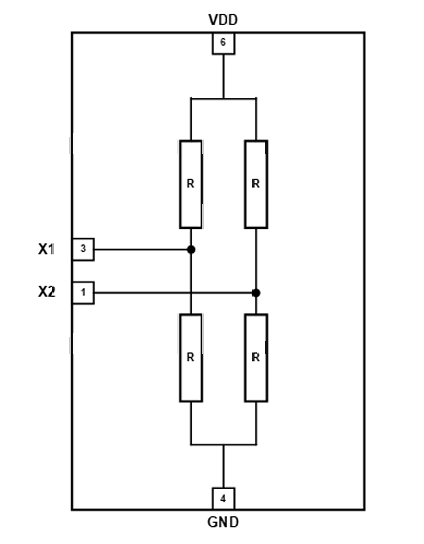
\includegraphics[height=6.5cm, keepaspectratio]{ct100-wheatstone.pdf.png}
    \\[3mm]
    \small (a) CT100 internal Wheatstone-bridge.
  \end{minipage}% <-- % prevents line break between minipages
  \hfill
  % --- RIGHT SIDE: Matched Circuit Schematic ---
  \begin{minipage}[b]{0.52\textwidth}
    \centering
    \begin{circuitikz}[american voltages, european resistors, scale=0.85, transform shape]
      
      % American DC Voltage Source (VDD) - 6 units tall
      \draw (0,0) to[american voltage source, invert, l=$V_{\text{DD}}$] (0,6)
            -- (2,6);
      \draw (0,0) -- (2,0);

      % Top & Bottom Rails with Connection Dots
      \draw (2,6) to[short, *-] (4,6);
      \draw (2,0) to[short, *-] (4,0);
      \draw (2,0) node[sground] {};

      % Left Bridge Leg (R1: 5.2 to 3.6, R3: 2.4 to 0.8)
      \draw (2,6) -- (2,5.2)
            to[R=$R_1$] (2,3.6)
            -- (2,2.4)
            to[R=$R_3$] (2,0.8)
            -- (2,0);

      % Right Bridge Leg (R2: 5.2 to 3.6, R4: 2.4 to 0.8)
      \draw (4,6) -- (4,5.2)
            to[R=$R_2$] (4,3.6)
            -- (4,2.4)
            to[R=$R_4$] (4,0.8)
            -- (4,0);

      % Output Line X1 (Tapped from left leg at y=3.2 with junction dot directly on x=2)
      \draw (2,3.2) to[short, *-o] (5.5,3.2) node[right] {$X_1$};

      % Output Line X2 (Tapped from right leg at y=2.8 with junction dot directly on x=4)
      \draw (4,2.8) to[short, *-o] (5.5,2.8) node[right] {$X_2$};

    \end{circuitikz}
    \\[3mm]
    \small (b) Equivalent bridge schematic.
  \end{minipage}

  \caption{Internal CT100 IC pin configuration alongside its labeled equivalent electrical schematic.}
  \label{fig:wheatstone_comparison}
\end{figure}


% 2. MATHEMATICAL DERIVATION SECOND
The CT100 arranges four internal TMR elements in a passive Wheatstone bridge configuration (Figure~\ref{fig:wheatstone_comparison}a). According to the device datasheet, the per-element resistance ranges from $R_{\min} \approx \SI{20}{\kilo\ohm}$ (parallel magnetic alignment, lowest-resistance state) to $R_{\max} \approx \SI{40}{\kilo\ohm}$ (antiparallel magnetic alignment, highest-resistance state). 

As a result of this Wheatstone-bridge configuration, the largest change in $V_{\text{out}}$ is $\frac{V_{\text{DD}}}{3}$:
\begin{equation}
    \Delta V_{\text{out,max}} = \frac{V_{\text{DD}}}{3}
\end{equation}
This maximum output swing is physically bounded by the internal TMR barrier resistance range ($R_{\min} \approx \SI{20}{\kilo\ohm}$ to $R_{\max} \approx \SI{40}{\kilo\ohm}$).

The voltage potentials at the two central output nodes, $X_1$ and $X_2$, as seen in Figure~\ref{fig:wheatstone_comparison}b are determined by the independent voltage divider ratios along the bridge:
\begin{equation}
    X_1 = V_{\text{DD}} \cdot \left( \frac{R_3}{R_1 + R_3} \right), \qquad X_2 = V_{\text{DD}} \cdot \left( \frac{R_4}{R_2 + R_4} \right)
    \label{eq:node_voltages}
\end{equation}

The general differential output voltage $V_{\text{out}}$ across nodes $X_1$ and $X_2$ is expressed as:
\begin{equation}
    V_{\text{out}} = X_1 - X_2 = V_{\text{DD}} \left( \frac{R_3}{R_1 + R_3} - \frac{R_4}{R_2 + R_4} \right)
    \label{eq:vout_general}
\end{equation}

At zero applied magnetic field ($B = \SI{0}{\tesla}$), all four TMR elements exhibit nominal, equal resistance ($R_1 = R_2 = R_3 = R_4$), yielding balanced potentials $X_1 = X_2 = \frac{V_{\text{DD}}}{2}$ and $V_{\text{out}} = \SI{0}{\volt}$. 

When an external magnetic field is applied along the sensitive axis, diagonal element pairs shift in opposing directions. One diagonal pair ($R_1, R_4$) decreases toward $R_{\min}$ while the opposite pair ($R_2, R_3$) increases toward $R_{\max}$. At full magnetic saturation, the resistance values reach their operational limits:
\begin{equation}
    R_1 = R_4 = R_{\min}, \quad \text{and} \quad R_2 = R_3 = R_{\max}
\end{equation}

Substituting these saturation values into Equation~\ref{eq:node_voltages} gives the node potentials at full saturation:
\begin{equation}
    X_{1,\text{sat}} = V_{\text{DD}} \cdot \left( \frac{R_{\max}}{R_{\min} + R_{\max}} \right), \qquad X_{2,\text{sat}} = V_{\text{DD}} \cdot \left( \frac{R_{\min}}{R_{\max} + R_{\min}} \right)
\end{equation}

Subtracting $X_{2,\text{sat}}$ from $X_{1,\text{sat}}$ yields the maximum theoretical differential output voltage $V_{\text{out,sat}}$:
\begin{equation}
    V_{\text{out,sat}} = X_{1,\text{sat}} - X_{2,\text{sat}} = V_{\text{DD}} \left( \frac{R_{\max} - R_{\min}}{R_{\max} + R_{\min}} \right)
    \label{eq:vout_sat_derived}
\end{equation}

Substituting the CT100 datasheet resistance values ($R_{\min} = \SI{20}{\kilo\ohm}$ and $R_{\max} = \SI{40}{\kilo\ohm}$):
\begin{equation}
    V_{\text{out,sat}} = V_{\text{DD}} \left( \frac{\SI{40}{\kilo\ohm} - \SI{20}{\kilo\ohm}}{\SI{40}{\kilo\ohm} + \SI{20}{\kilo\ohm}} \right) = V_{\text{DD}} \left( \frac{20}{60} \right) = \frac{V_{\text{DD}}}{3}
\end{equation}

This  derivation proves that the maximum differential output voltage is  bound to $\frac{V_{\text{DD}}}{3}$. For a supply voltage of $V_{\text{DD}} = \SI{3.30}{\volt}$, the theoretical saturation output is $ \SI{1.10}{\volt}$, which aligns with the experimentally measured saturation output of $\SI{1.12}{\volt}$ reported in Section~\ref{sec:standalone-sat-recovery}.

% 3. DEFINITION STATEMENT THIRD
\textbf{Furthermore}, from this point forward in this report, the sensor's output voltage is defined as \textbf{$V_{\text{out}} = X_1 - X_2$}, which was applied  across all DMM, oscilloscope, and MCU measurement in this work.


\section{Available Instrumentation}
\label{sec:instrumentation}

Characterization and bench-top tests were conducted using the following laboratory equipment to ensure power delivery and take measurements.

\begin{itemize}
    \item \textbf{Digital Oscilloscope:} Rohde \& Schwarz RTB2002 (\SI{2.5}{GS/s} sampling rate, 10-bit A/D converter) for transient analysis, step-response monitoring across nodes \(X_1\) and \(X_2\).
    \item \textbf{ Digital Multimeter (DMM):} Keithley 2110 \(5\frac{1}{2}\) Digit Dual-Display Multimeter for DC Voltage and Current logging and cross-validating MCU reading accuracy.
    
    \item \textbf{DC Power Supply Unit (PSU):} Topward dual-tracking linear DC power supply capable of supplying up to \SI{6.0}{\ampere} continuously, providing supply voltage  and current excitation through the PCB test trace.
    
    \end{itemize}

\section{Standalone Sensor Board}
\label{sec:standalone-board}

\subsection{PCB Design}
\label{sec:standalone-pcb}

A standalone sensor board was designed in Altium Designer containing only the CT100 sensor and a single \SI{0.1}{\micro\farad} decoupling capacitor.

The board is driven directly from a laboratory power supply, with the  differential outputs ($X_1, X_2$) routed directly to a digital oscilloscope and digital multimeter (DMM). Signal amplification was deliberately excluded from this characterization topology. Although raw bridge differential voltages can be relatively small, avoiding amplifier stages eliminates amplifier constraints—such as slew rate and  bandwidth obscuring the true recovery time of the TMR bridge itself. Probing the unconditioned Wheatstone output directly establishes a true baseline of the sensor's native sensitivity and saturation recovery. This design was used in Daniel Tieu's work on Thermal Cycling.

The PCB can be seen in Figure 3 below.


\subsection{Saturation Testing Methodology}
\label{sec:sat-test-methodology}

For this board, saturation was induced using an external Neodymium magnet ($> \SI{110}{\milli\tesla}$), manually brought toward and away from the sensor. This was the simplest available stimulus for an initial characterisation but is not repeatable or automatable; its limitations, 

\subsection{Sensor-Only Saturation and Recovery Behaviour}
\label{sec:standalone-sat-recovery}

With no applied field, the differential output ($V_{\text{out}} = X1-X2$) sits at a near-zero baseline of \SI{4.5087}{\milli\volt} (Figure~\ref{fig:scope}). As the field increases past approximately \SI{20.0}{\milli\tesla}, the bridge output plateaus at a fixed differential ceiling of \SI{1.12}{\volt}, matching the $V_{\text{CC}}/3$ derivation in Section~\ref{sec:bridge-topology}, and never rails to the $V_{\text{CC}}$ supply itself.

\begin{figure}[h]
\centering
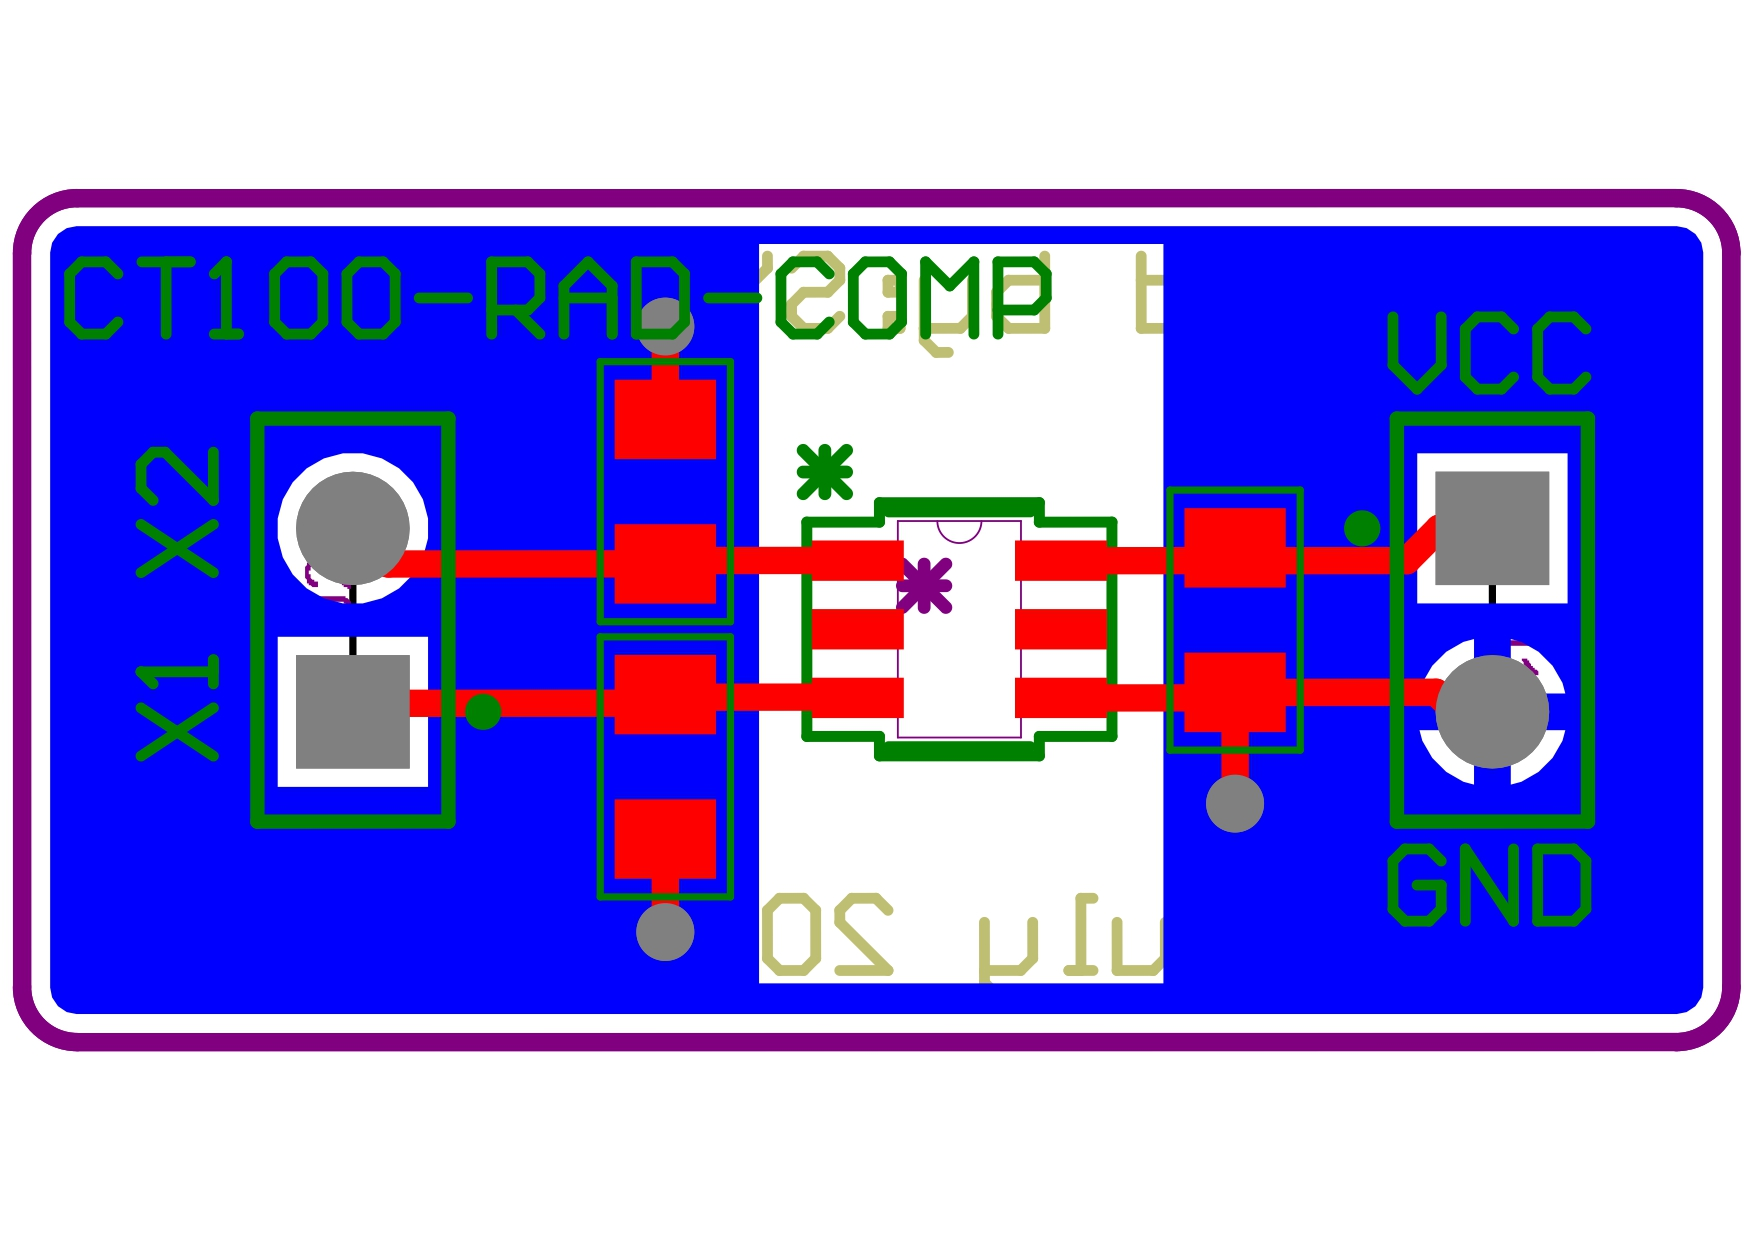
\includegraphics[width=0.7\textwidth]{TMR_RAD_COMPARE_page-0001.jpg}
\caption{Standalone Sensor PCB}
\label{fig:scope}
\end{figure}


\begin{figure}[h]
\centering
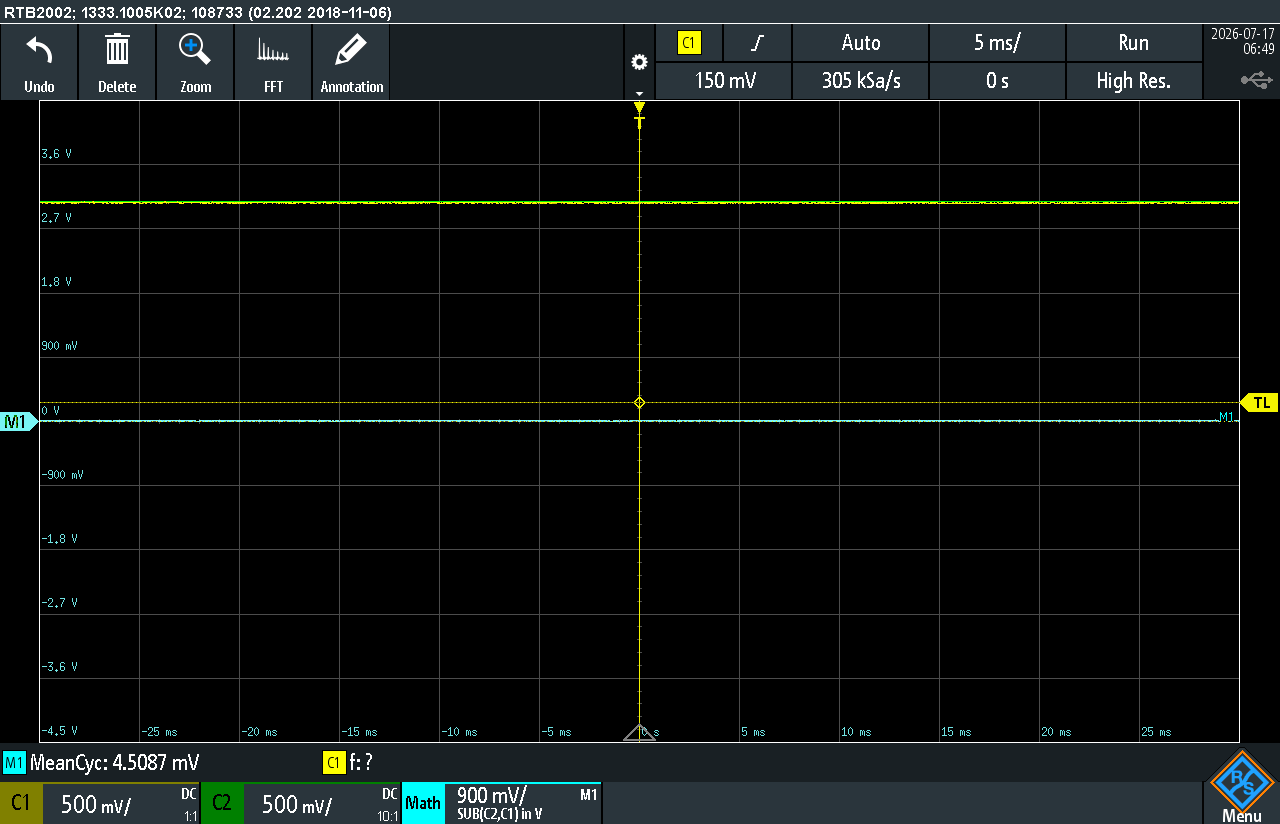
\includegraphics[width=0.7\textwidth]{scope_x1-x2_compare_code.PNG}
\caption{Isolated-board saturation characteristics}
\label{fig:scope}
\end{figure}

Recovery time back to baseline after saturation was  quantified  ( \SI{82.3}{\milli\second}, \textasciitilde\SI{12.15}{\hertz}) 

\todo{add scope image of saturation response time
} This recovery frequency is directly relevant to CubeSat operation: if the OBC's magnetometer sampling rate is high relative to the sensor's recovery frequency, a sample taken shortly after a magnetorquer pulse risks capturing the sensor mid-recovery rather than the true ambient field, so ADCS software must budget a guardband around any magnetorquer firing before trusting the next magnetometer reading. \todo{Insert a specific guardband calculation once a target OBC sampling frequency is defined.}


\textbf{Hysteresis.} \todo{This subsection reports a finding stated during testing that has not yet been fully quantified or reconciled against the "instant return to baseline" observation above -- please confirm the following before it goes into a final submission.} Once driven into saturation, the sensor was observed to return to a \emph{new}, offset baseline rather than the original zero-field value, with the output remaining linear about this new offset for subsequent field excursions. This is consistent with magnetic hysteresis in the free layer: after saturation, the free layer's magnetisation does not fully relax back to its original zero-field orientation, leaving a small permanent shift in the balance point of the bridge. \todo{Quantify the magnitude of this offset (mV), confirm whether it is stable over time/repeated cycles, and clarify which board/session this was observed on, since it appears to sit alongside an earlier record of the output returning "instantly" to the original linear baseline after saturation -- these two observations should be reconciled (e.g.\ the earlier note may have predated the sensor's first-ever saturation, with hysteresis only appearing from the first saturation event onward).} This has a direct design implication aligns with current research state it and talk about implications of why it would be bad.




\section{Integrated Board: Field Excitation and Design}
\label{sec:integrated-board}

\subsection{Integrated Board Design}
\label{sec:integrated-design}

To accurately characterize the sensor's sensitivity without relying solely on a handheld neodymium magnet, a repeatable and quantifiable test field was required.

A current-carrying PCB trace routed directly beneath the sensor die was selected. This DC current induces a magnetic field around the trace that acts upon the TMR sensor to generate a measurable voltage output. Its generated magnetic field is calculated analytically and simulated in Ansys Maxwell, serving as a theoretical benchmark for expected sensor output against practical results. The trace current can be swept up to the laboratory PSU's \SI{6.0}{\ampere} limit. 

While the upper limit of the PSU capability \SI{6.0}{\ampere}  does not generate a strong enough magnetic field to drive the CT100 into full saturation, it provides a linear sweep to determine the sensor's sensitivity. Establishing this sensitivity benchmark is critical as later in the characterization, when the sensor is deliberately driven to saturation, this baseline allows us to measure any resulting hysteresis, zero-point drift, or degradation in linearity.

The system architecture of the integrated board revolves around three core components to emulate the final operational environment and precisely back-calculate the applied magnetic field:

\begin{itemize}
    \item \textbf{Microcontroller (MCU):} Ane STM32G431KBT6 was selected for its high-performance. The CT100 differential output pair feeds the MCU's internal differential ADC channels directly, sampled at \SI{1.0}{\kilo\hertz}. The MCU features a 12-bit ADC andl auto-calibration routines were run to minimise discrepancies between ADC's on MCU on different boards.
    
    \item \textbf{Current Monitor (INA219):} Because the PSU's analog display was not trusted as precise means of determining current, a dedicated INA current-sense with a Kelvin-connected \( \SI{5.0}{\milli\ohm}\) shunt resistor. This was used to back-calculate the magnetic field generated by the trace current acting on the TMR sensor.
    
    \item \textbf{Low-Dropout (LDO) regulator:} The board is powered via a \SI{5.0}{\volt} input rail which is fed into into a LDO regulator to provide a clean \SI{3.30}{\volt} supply to both the sensor and MCU. This LDO also provides a high Power Supply Rejection Ratio (PSRR) and sets the subsequent resolution of the TMR sensor. 
    
\end{itemize}


As shown in Figure~\ref{fig:board}, the current carrying trace is routed on the bottom layer (highlighted in blue). The corresponding circuit schematic clarifies the positive current ($+i$) sign convention adopted for all subsequent field calculations and experimental sweeps. The schematic for this design can be found in the Appendix A.

\begin{figure}[h]
\centering
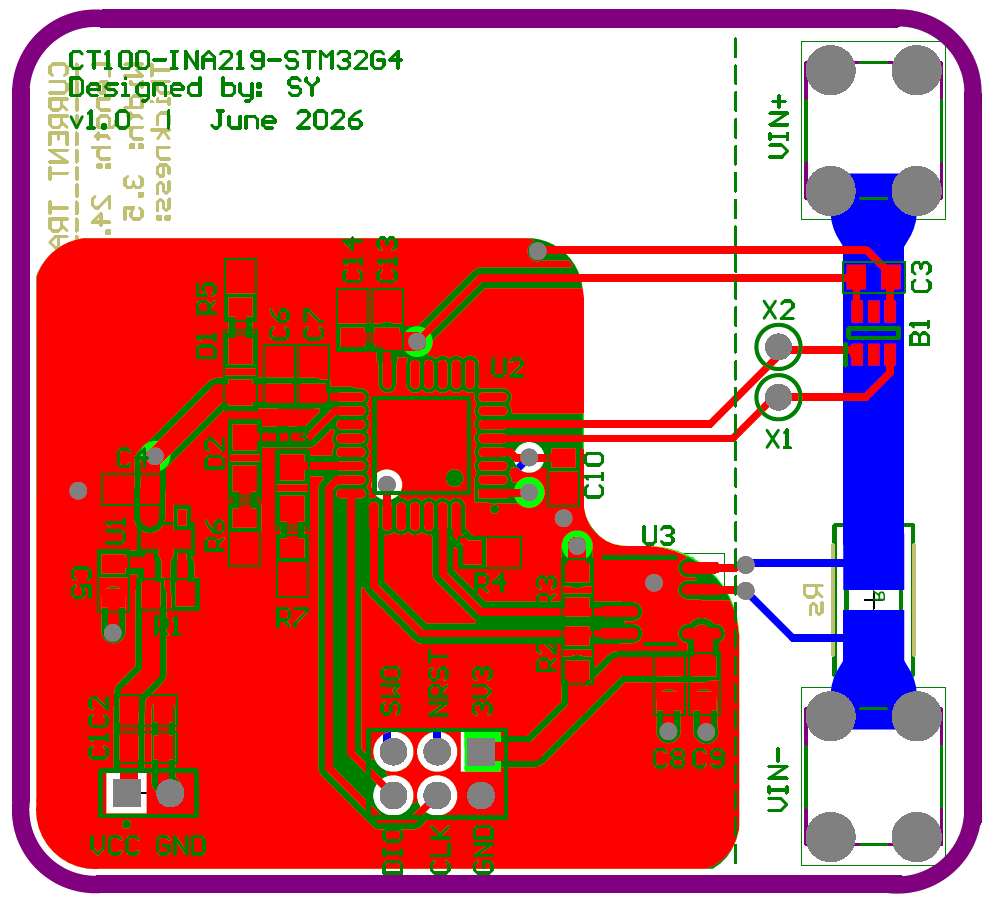
\includegraphics[width=0.47\textwidth]{magsat_layout.png}\hfill
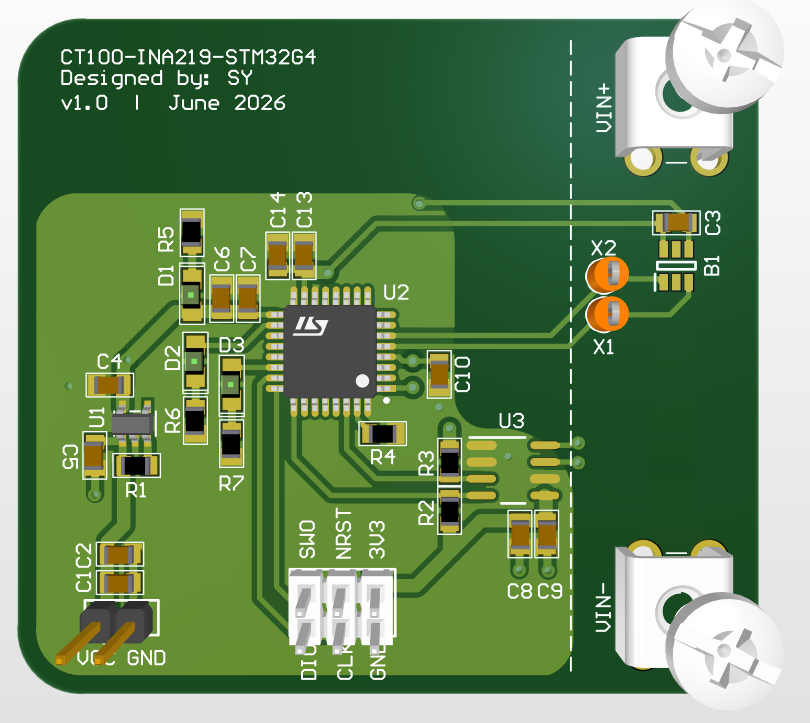
\includegraphics[width=0.47\textwidth]{magsat_pcb_front.png}
\caption{Integrated board layout (left) and rendered assembly view (right).}
\label{fig:board}
\end{figure}

\begin{figure}[htbp]
\centering

\begin{circuitikz}[scale=1.1, transform shape]
    % Terminals on the right using standard path poles (-o)
    \draw (3,3) to[short, -o] (5,3) node[right] {\textbf{\(V_{\text{IN}}^+\)}};
    \draw (3,0) to[short, -o] (5,0) node[right] {\textbf{\(V_{\text{IN}}^-\)}};

    % Top horizontal rail with leftward positive current arrow (+i)
    \draw (3,3) to[short, i_=\(+i\)] (0,3);

    % Bottom horizontal rail
    \draw (0,0) -- (3,0);

    % Middle vertical branch: Upward Current Source (i)
    \draw (3,0) to[american current source, l_=\(i\)] (3,3);

    % Junction nodes at the T-connections (filled dots)
    \node[circ] at (3,3) {};
    \node[circ] at (3,0) {};

    % Far-left branch: European Resistor R_shunt
    \draw (0,3) to[R, european, l_=\(R_{\text{shunt}}\)] (0,0);

\end{circuitikz}
\caption{Field excitation circuit schematic and positive trace current convention (\(+i\)).}
\label{fig:excitation_circuit}
\label{fig:excitation_schematic_v2}
\end{figure}

\subsection{PCB Trace Design}
\label{sec:pcb-trace}

The current-carrying trace was routed on a custom four-layer PCB, with layer thicknesses and dielectric parameters detailed in Table~\ref{tab:stackup}. To avoid distorting the magnetic field induced by the current trace the TMR sensor, no copper pour was placed near the TMR sensor besides the PCB trace. The trace was routed such that current flow produces a field acting on the sensor's most senstiive axis. 

\begin{table}[h]
\centering
\caption{Four-layer PCB stack-up specification.}
\label{tab:stackup}
\begin{tabular}{@{}lllr@{}}
\toprule
Layer & Material & Copper Weight & Thickness \\
\midrule
Top Solder & Solder Mask (SM-001) & --- & \SI{0.0254}{\milli\metre} \\
Top Layer & Signal Conductor (CF-004) & 1.0 oz & \SI{0.0350}{\milli\metre} \\
Layer 2 (GND) & Signal Conductor (CF-001) & 0.25 oz & \SI{0.0090}{\milli\metre} \\
Layer 3 (PWR) & Signal Conductor (CF-001) & 0.25 oz & \SI{0.0090}{\milli\metre} \\
Bottom Layer & Signal Conductor (CF-004) & 1.0 oz & \SI{0.0350}{\milli\metre} \\
Bottom Solder & Solder Mask (SM-001) & --- & \SI{0.0254}{\milli\metre} \\
\bottomrule
\end{tabular}
\end{table}

This stack-up yields a total conductive copper thickness of \SI{0.08799}{\milli\metre}, a dielectric core height of \SI{0.8382}{\milli\metre}, and an overall board thickness of \SI{0.97699}{\milli\metre}. The excitation trace is routed on the bottom layer with a track width \(w = \SI{3.5}{\milli\metre}\), capable of currents up to the PSU's \SI{6.0}{\ampere} limit.


\subsection{Analytical Field Model}
\label{sec:field-model}

The horizontal magnetic field at the TMR die height (\(d = \SI{0.4229}{\milli\metre}\)) beneath the centre of the trace (\(w = \SI{3.5}{\milli\metre}\)) is modelled using the standard planar-strip-conductor formulation:
\begin{equation}
B_{\text{planar}} = \mu_0 \left[ \frac{I}{\pi w} \arctan\left( \frac{w}{2d} \right) \right].
\label{eq:planar}
\end{equation}
Evaluated at a trace current of \(I = \SI{4.175}{\ampere}\), this analytical model yields a theoretical flux density of \SI{462.70}{\micro\tesla}.

\subsection{Simulated vs.\ Experimental Field Validation}
\label{sec:field-validation}

The analytical field model was cross-checked against a finite-element simulation in Ansys Maxwell. The simulation resolves the full 3D near-field map around the trace rather than the simplified 2D geometry assumed by Equation~\eqref{eq:planar} the Ansys model can be seen in  Figure~\ref{fig:ansys}. The two models align closely the simulation outputted \(\approx\SI{500}{\micro\tesla}\) simulated at \SI{4.175}{\ampere} while the analytical solution gave \SI{462.70}{\micro\tesla} analytically, the formula appears to be a close approximation for the 3D simulation at this geometry. 

An experiment was conducted to compare any discrepancies between our analytical and experimental results. We measured the output voltage at \SI{4.175}{\ampere} to be \(\approx\SI{16}{\milli\volt}\) using a DMM. Which was roughly double what the simulatation predicted \(\approx\SI{7.43}{\milli\volt}\) . This discrepancy, and its possible causes; external ambient field offsets is examined in Section~\ref{sec:shielding}.

\begin{figure}[h]
\centering
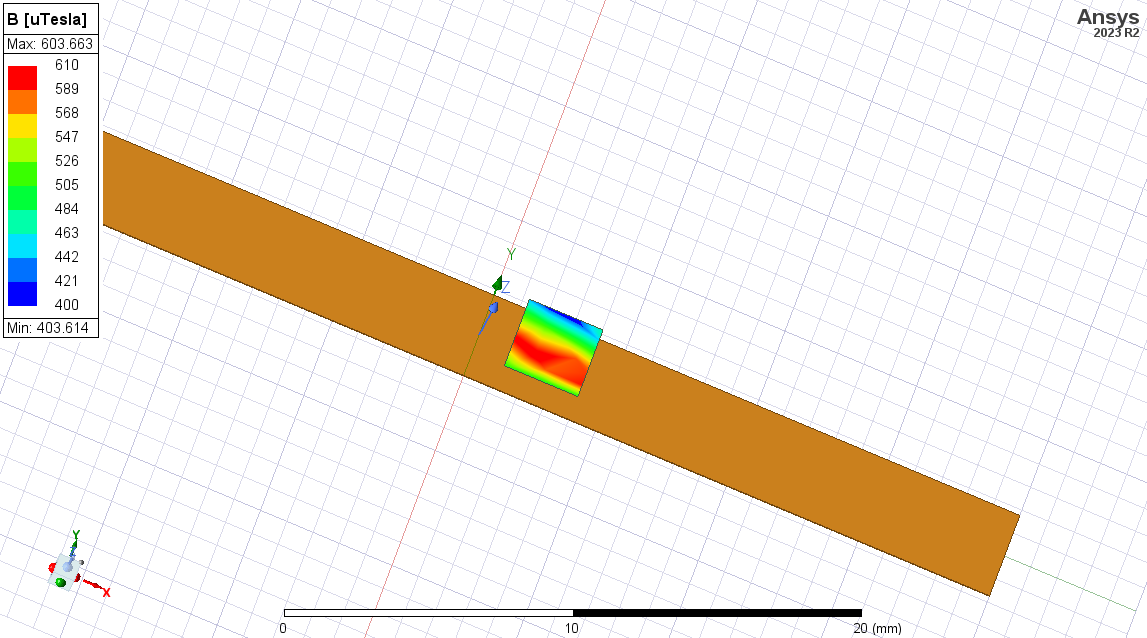
\includegraphics[width=0.75\textwidth]{anys_trace.png}
\caption{Ansys near-field simulation of the current trace.}
\label{fig:ansys}
\end{figure}



\subsection{Firmware}
\label{sec:firmware}

The firmware is built upon the STM32 Hardware Abstraction Layer (HAL). The MCU's ADC is configured in differential-pair mode, sampling \(X_1 - X_2\) directly and converting the raw 12-bit value to volts via:
\begin{equation}
X_1 - X_2 = \left( \frac{\text{ADC}_{\text{raw}} - 2048}{2048} \right) \times V_{\text{DD}}
\label{eq:adcconv}
\end{equation}
where 2048 is the mid-scale ADC code corresponding to the zero-differential (balanced-bridge) midpoint. Hardware ADC self-calibration (\texttt{HAL\_ADCEx\_Calibration\_Start}) is executed automatically on every boot before any conversions occur. The MCU continuously polls the INA219 over \(\text{I}^2\text{C}\) for trace current and streams both the current and voltage values out in real time over the Serial Wire Viewer (SWV) debug channel for offline analysis in MATLAB. The code can be found in Appendix B.


\subsection{Design Note for Future PCB Revisions}
\label{sec:future-pcb-note}

Because the sensor bridge is nominally balanced at \(V_{\text{DD}}/2\) (Section~\ref{sec:bridge-topology}), the ADC channel monitoring it spends its full dynamic range on either side of that midpoint. Any measurement taken near the zero-differential code inherits the ADC's own quantization and calibration uncertainty around that center point (see the code-1042 fault discussed in Section~\ref{sec:instr-validation}). 

A future PCB revision could integrate a hardware offset to bias the bridge's reference point to a non-zero value. This is expected to (i) reduce measurement error introduced by operating close to the ADC's most quantization-sensitive midpoint code, and (ii) artificially reduce the external magnetic field magnitude required to drive the sensor to its effective saturation bounds for testing purposes. \todo{This is currently a design intention rather than a tested result -- expand with the specific biasing approach and expected numbers if it is implemented on a future board revision.}



\section{Non-Irradiated Sensitivity and Saturation Characterisation}
\label{sec:nonirr-characterisation}

\subsection{Data Collection Method}
\label{sec:data-collection}

Current-sweep data was logged via the MCU's SWV output, exported, and processed in MATLAB. Rather than relying on single instantaneous readings, each current setting was captured over a 20-second window and averaged. A single-sample readings were found to be unreliable due to the  MCU ADC's quantisation behaviour where raw SWV data at a given current setting was observed hopping between a small number of discrete levels spaced at multiples of the \SI{1.61}{\milli\volt} LSB typically spanning 1--2 LSBs of scatter around the true mean.


\subsection{Saturation Recovery on the Integrated Board}
\label{sec:sat-recovery-integrated}

On the integrated board, with a regulator input of $V_{\text{CC}} = \SI{4.97}{\volt}$ and a TMR sensor supply of $V_{\text{DD}} = \SI{3.32}{\volt}$, the saturation-to-baseline voltage swing was $\Delta V = \SI{1.1521}{\volt}$, with a recovery time of $t_{\text{rec}} = \SI{82.3}{\milli\second}$, corresponding to a recovery frequency of $f \approx \SI{12.15}{\hertz}$ (Figure~\ref{fig:swv}).

\begin{figure}[h]
\centering
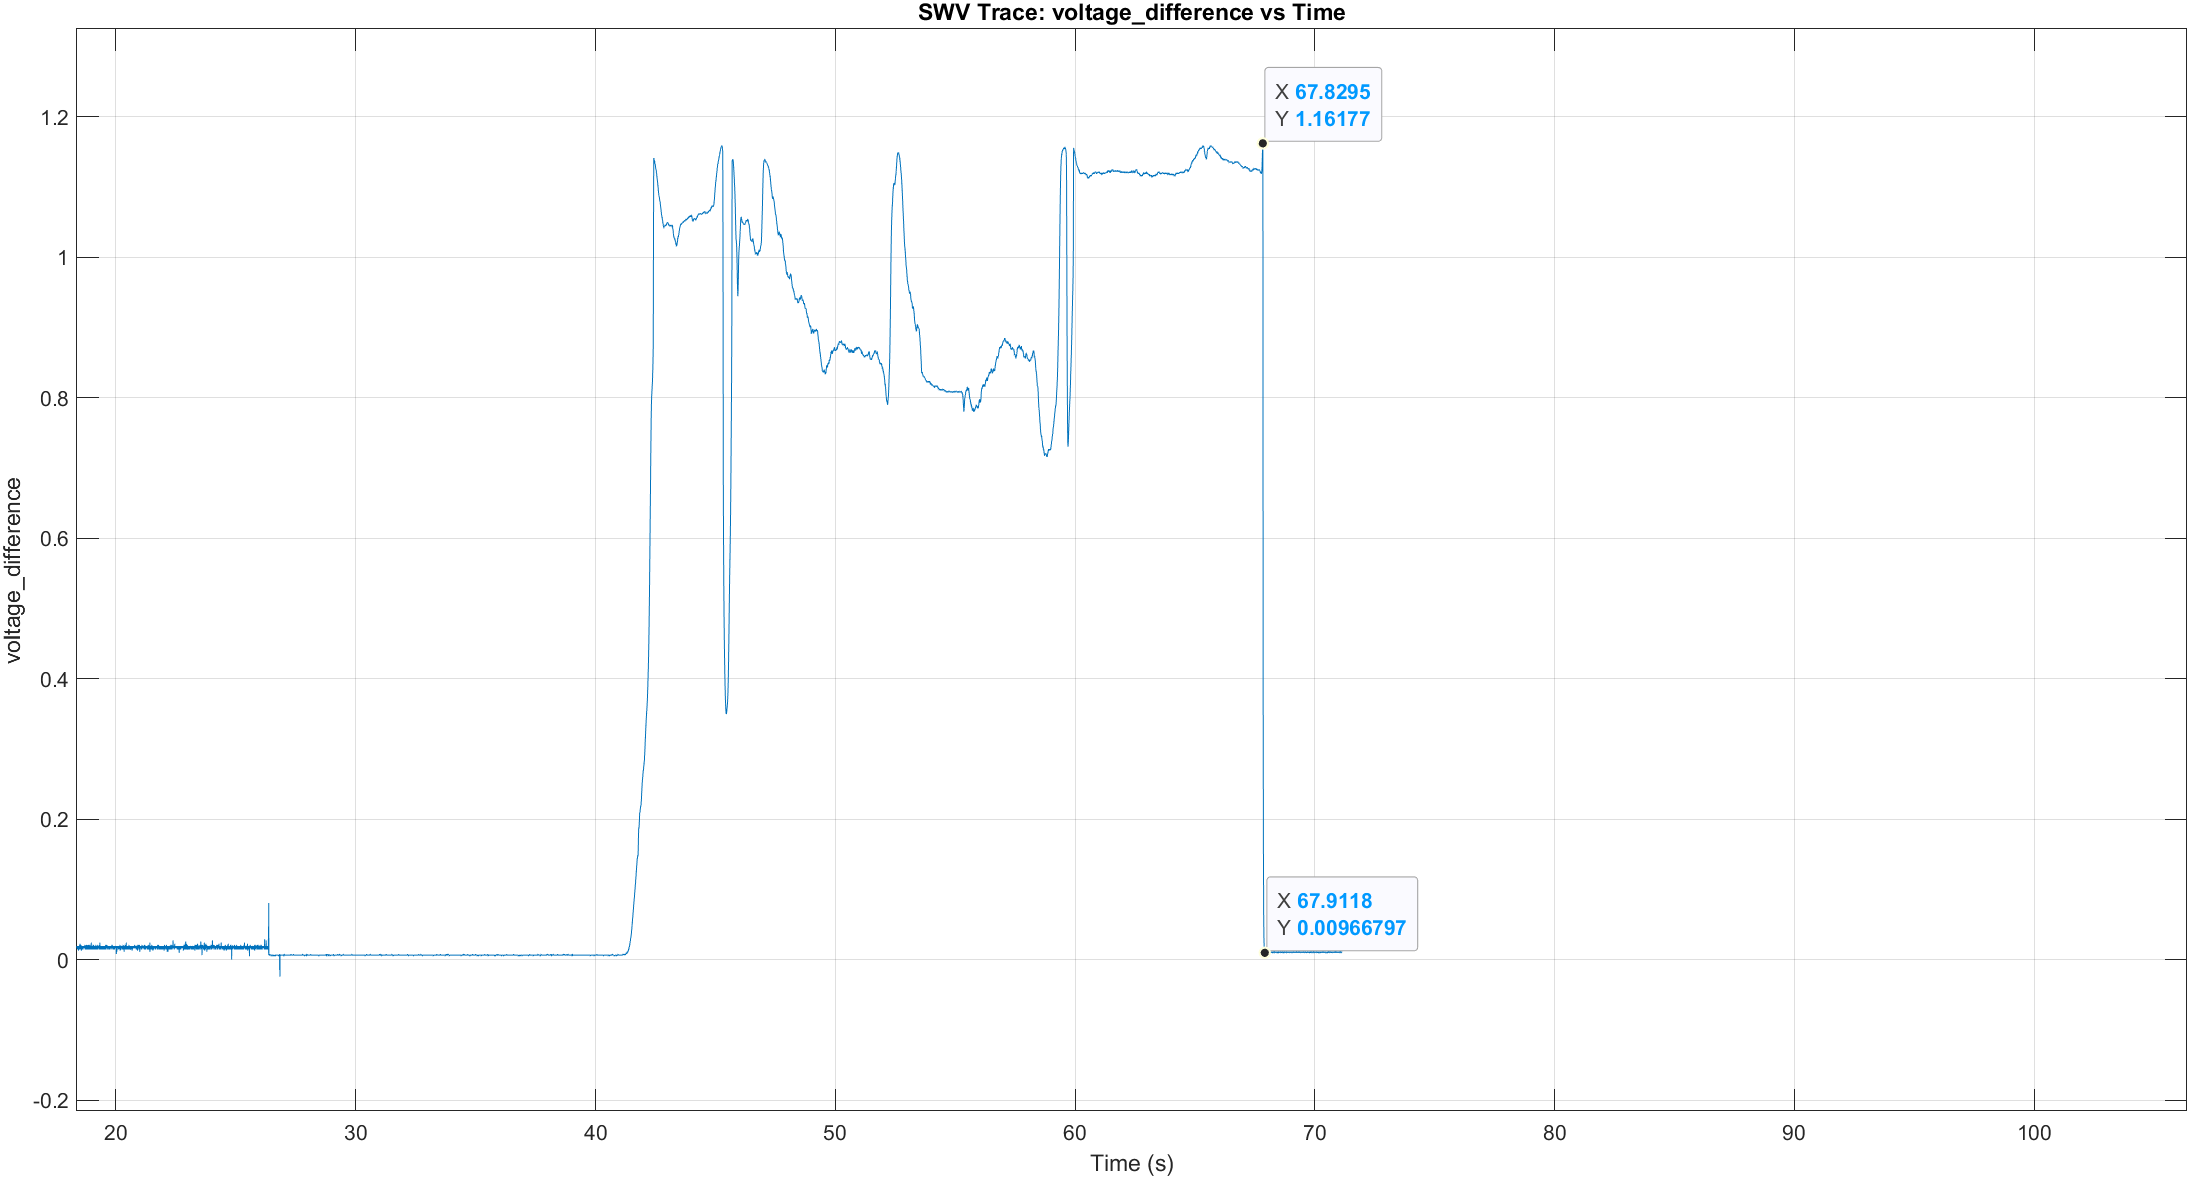
\includegraphics[width=0.85\textwidth]{response.png}
\caption{Measured saturation recovery response on the integrated board (SWV trace, logged and plotted in MATLAB).}
\label{fig:swv}
\end{figure}

\subsection{Current Sweep: Data and Sensitivity Fit}
\label{sec:sensitivity-fit}

The trace current was swept from $-3.0$ to $+\SI{3.0}{\ampere}$ in approximately \SI{0.5}{\ampere} steps, all within a single session at $V_{\text{CC}} = \SI{3.30}{\volt}$ (Table~\ref{tab:sensitivity-unirr-full}).

\begin{table}[H]
    \centering
    \small 
    \caption{Non-Irradiated \&\ No Shielding Current Sweep Data}
    \label{tab:sensitivity-unirr-full}
    % CHANGED: 'ccccc' forces all columns to center alignment
    \begin{tabular}{@{}ccccc@{}}
        \toprule
        DMM Current (mA) & INA Current (mA) & DMM (mV) & MCU (mV) & Scope (mV) \\
        \midrule
        \(-2991.0\) & \(-2966.7\) & 8.634 & 8.069 & \(-12.207\) \\
        \(-2498.5\) & \(-2478.2\) & 9.860 & 9.571 & \(-10.986\) \\
        \(-2029.0\) & \(-2012.6\) & 9.950 & 9.584 & \(-10.376\) \\
        \(-1501.0\) & \(-1487.7\) & 11.690 & 11.249 & \(-9.766\) \\
        \(-1022.0\) & \(-1016.6\) & 11.250 & 11.107 & \(-9.308\) \\
        \(-499.0\) & \(-498.2\) & 12.650 & 12.022 & \(-10.681\) \\
        \(-0.7\) & \(-6.3\) & 12.980 & 12.847 & \(-8.594\) \\
        $499.0$ & 487.8 & 14.450 & 13.628 & \(-7.477\) \\
        $1022.0$ & 1005.2 & 14.210 & 13.796 & \(-5.035\) \\
        $1501.0$ & 1477.2 & 15.697 & 14.790 & \(-6.104\) \\
        $2029.0$ & 2002.1 & 15.720 & 15.020 & \(-3.516\) \\
        $2498.5$ & 2466.4 & 16.500 & 16.068 & \(-3.906\) \\
        $2991.0$ & 2954.8 & 16.570 & 16.088 & \(-5.030\) \\
        \bottomrule
    \end{tabular}
\end{table}

A linear fit of bridge output against trace current gives a sensitivity of
\SI{1.356}{\milli\volt\per\ampere} on the DMM ($R^2 = 0.974$) and
\SI{1.315}{\milli\volt\per\ampere} on the MCU ($R^2 = 0.981$).

The CT100 datasheet specifies a typical full-bridge sensitivity of
\SI{4.5}{\milli\volt\per\volt\per\milli\tesla}, with a specified range of
\SI{3.8}{\milli\volt\per\volt\per\milli\tesla} to
\SI{5.2}{\milli\volt\per\volt\per\milli\tesla}. At the
\SI{3.30}{\volt} supply voltage used for this characterisation, the
corresponding theoretical voltage sensitivity is therefore

\begin{equation}
S_{V,\mathrm{theory}}
=
S_{\mathrm{CT100}}V_{\mathrm{DD}}
=
\left(\SI{4.5}{\milli\volt\per\volt\per\milli\tesla}\right)
\left(\SI{3.30}{\volt}\right)
=
\SI{14.85}{\milli\volt\per\milli\tesla}.
\label{eq:ct100-voltage-sensitivity}
\end{equation}

The analytical field model in Equation~\eqref{eq:planar} gives a field
coefficient of approximately
\SI{0.1108}{\milli\tesla\per\ampere} for the trace geometry used in the
test. Combining this field response with the CT100 sensitivity gives the
expected voltage change per unit trace current:

\begin{equation}
\frac{\mathrm{   \Delta}V_{\mathrm{out}}}{\mathrm{   \Delta}I}
=
S_{V,\mathrm{theory}}
\frac{\mathrm{   \Delta}B}{\mathrm{   \Delta}I}
=
\left(\SI{14.85}{\milli\volt\per\milli\tesla}\right)
\left(\SI{0.1108}{\milli\tesla\per\ampere}\right)
=
\SI{1.645}{\milli\volt\per\ampere}.
\label{eq:ct100-voltage-current-slope}
\end{equation}

Thus, for a given trace current, the theoretical sensor output can be
written as

\begin{equation}
V_{\mathrm{out,theory}}
=
V_0
+
\left(\SI{1.645}{\milli\volt\per\ampere}\right)I,
\label{eq:ct100-expected-voltage}
\end{equation}

where $V_0$ is the zero-field output voltage. Figure~\ref{fig:voltage-cross-val} below 
uses a $V_0$ value of \SI{12.980}{\milli\volt} to visually compare the voltage
\emph{slope}; it is not a theoretical prediction of the CT100 offset voltage.

For comparison with the measured slopes, the DMM result corresponds to

\begin{equation}
S_{\mathrm{DMM}}
=
\frac{\SI{1.356}{\milli\volt\per\ampere}}
{\SI{0.1108}{\milli\tesla\per\ampere}
\times \SI{3.30}{\volt}}
=
\SI{3.71}{\milli\volt\per\volt\per\milli\tesla},
\end{equation}

while the MCU result corresponds to
\SI{3.60}{\milli\volt\per\volt\per\milli\tesla}. The DMM-based value is
therefore approximately $17.6\%$ below the typical datasheet value of
\SI{4.5}{\milli\volt\per\volt\per\milli\tesla}, while the MCU-based value
is approximately $20.1\%$ below it. The DMM result is also only slightly
below the datasheet's specified minimum of
\SI{3.8}{\milli\volt\per\volt\per\milli\tesla}.

\begin{figure}[H]
    \centering

    % ============================================================
    % LEFT: Voltage Plot
    % ============================================================
    \begin{minipage}[t]{0.48\textwidth}
        \centering

        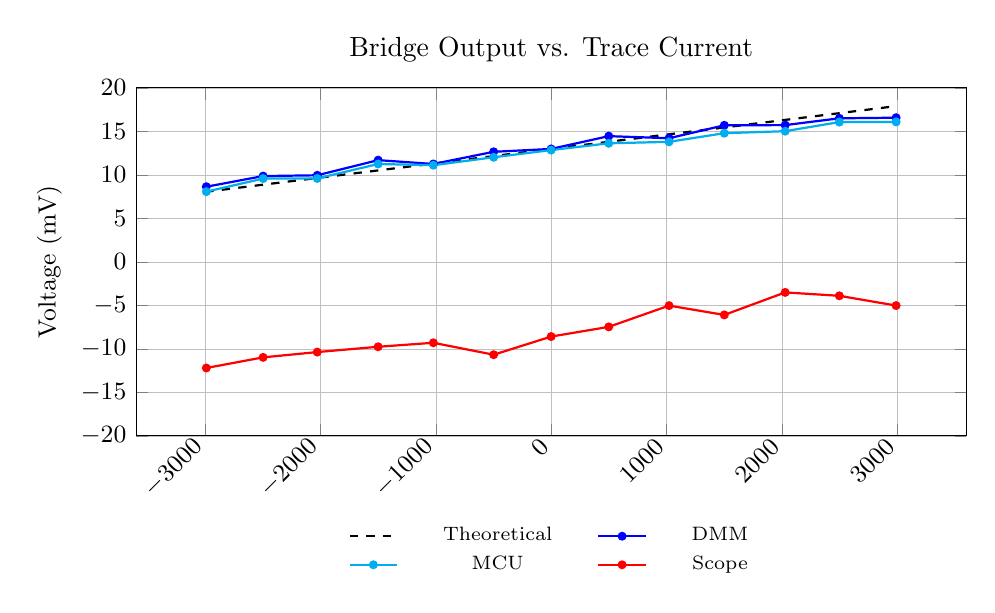
\begin{tikzpicture}
            \begin{axis}[
                width=\textwidth,
                height=6cm,
                title={Bridge Output vs. Trace Current},
                xlabel={Current (mA)},
                ylabel={Voltage (mV)},
                grid=both,
                grid style={line width=.1pt, draw=gray!20},
                major grid style={line width=.2pt, draw=gray!50},
                mark size=1.2pt,
                xtick={-3000,-2000,-1000,0,1000,2000,3000},
                x tick label style={rotate=45, anchor=east},
                /pgf/number format/1000 sep={},
                label style={font=\small},
                tick label style={font=\small},
                legend style={
                    at={(0.5,-0.23)},
                    anchor=north,
                    font=\scriptsize,
                    legend columns=2,
                    /tikz/column sep=0.5cm,
                    draw=none
                },
          ymin=-20,
ymax=20,
ytick={-20,-15,-10,-5,0,5,10,15,20},
            ]

                % ------------------------------------------------
                % Theoretical response
                %
                % CT100 sensitivity = 4.5 mV/V/mT
                % VDD = 3.30 V
                % Analytical field coefficient = 0.1108 mT/A
                %
                % dV/dI = 4.5 x 3.30 x 0.1108
                %       = 1.645 mV/A
                %
                % 12.980 mV is used only as a visual intercept
                % to compare slope with the measured response.
                % ------------------------------------------------
                \addplot[
                    color=black,
                    dashed,
                    thick,
                    domain=-3000:3000,
                    samples=100
                ]
                {12.980+1.64538*(x/1000)};
                \addlegendentry{Theoretical}

                % ------------------------------------------------
                % DMM Data
                % ------------------------------------------------
                \addplot[
                    color=blue,
                    thick,
                    mark=*
                ]
                coordinates {
                    (-2991.0, 8.634)
                    (-2498.5, 9.860)
                    (-2029.0, 9.950)
                    (-1501.0, 11.690)
                    (-1022.0, 11.250)
                    (-499.0, 12.650)
                    (-0.7, 12.980)
                    (499.0, 14.450)
                    (1022.0, 14.210)
                    (1501.0, 15.697)
                    (2029.0, 15.720)
                    (2498.5, 16.500)
                    (2991.0, 16.570)
                };
                \addlegendentry{DMM}

                % ------------------------------------------------
                % MCU Data
                % ------------------------------------------------
                \addplot[
                    color=cyan,
                    thick,
                    mark=*
                ]
                coordinates {
                    (-2991.0, 8.069)
                    (-2498.5, 9.571)
                    (-2029.0, 9.584)
                    (-1501.0, 11.249)
                    (-1022.0, 11.107)
                    (-499.0, 12.022)
                    (-0.7, 12.847)
                    (499.0, 13.628)
                    (1022.0, 13.796)
                    (1501.0, 14.790)
                    (2029.0, 15.020)
                    (2498.5, 16.068)
                    (2991.0, 16.088)
                };
                \addlegendentry{MCU}

                % ------------------------------------------------
                % Scope Data
                % ------------------------------------------------
                \addplot[
                    color=red,
                    thick,
                    mark=*
                ]
                coordinates {
                    (-2991.0, -12.207)
                    (-2498.5, -10.986)
                    (-2029.0, -10.376)
                    (-1501.0, -9.766)
                    (-1022.0, -9.308)
                    (-499.0, -10.681)
                    (-0.7, -8.594)
                    (499.0, -7.477)
                    (1022.0, -5.035)
                    (1501.0, -6.104)
                    (2029.0, -3.516)
                    (2498.5, -3.906)
                    (2991.0, -5.030)
                };
                \addlegendentry{Scope}

            \end{axis}
        \end{tikzpicture}

        \captionof{figure}{
            Voltage cross-validation during the non-irradiated, unshielded
            current sweep. The dashed line shows the theoretical CT100
            response.
        }
        \label{fig:voltage-cross-val}

    \end{minipage}%
    \hfill
    % ============================================================
    % RIGHT: Current Cross-Validation
    % ============================================================
    \begin{minipage}[t]{0.48\textwidth}
        \centering

        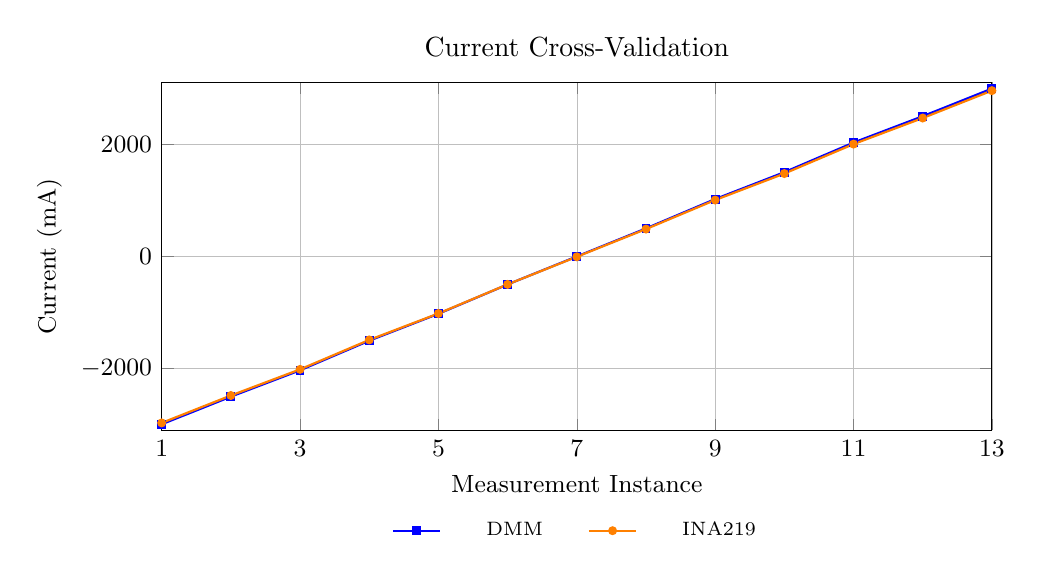
\begin{tikzpicture}
            \begin{axis}[
                width=\textwidth,
                height=6cm,
                title={Current Cross-Validation},
                xlabel={Measurement Instance},
                ylabel={Current (mA)},
                grid=both,
                grid style={line width=.1pt, draw=gray!20},
                major grid style={line width=.2pt, draw=gray!50},
                mark size=1.2pt,
                xmin=1,
                xmax=13,
                xtick={1,3,5,7,9,11,13},
                /pgf/number format/1000 sep={},
                label style={font=\small},
                tick label style={font=\small},
                legend style={
                    at={(0.5,-0.23)},
                    anchor=north,
                    font=\scriptsize,
                    legend columns=2,
                    /tikz/column sep=0.5cm,
                    draw=none
                },
                ymin=-3100,
                ymax=3100
            ]

                % ------------------------------------------------
                % DMM Current
                % ------------------------------------------------
                \addplot[
                    color=blue,
                    thick,
                    mark=square*
                ]
                coordinates {
                    (1,-2991.0)
                    (2,-2498.5)
                    (3,-2029.0)
                    (4,-1501.0)
                    (5,-1022.0)
                    (6,-499.0)
                    (7,-0.7)
                    (8,499.0)
                    (9,1022.0)
                    (10,1501.0)
                    (11,2029.0)
                    (12,2498.5)
                    (13,2991.0)
                };
                \addlegendentry{DMM}

                % ------------------------------------------------
                % INA219 Current
                % ------------------------------------------------
                \addplot[
                    color=orange,
                    thick,
                    mark=*
                ]
                coordinates {
                    (1,-2966.7)
                    (2,-2478.2)
                    (3,-2012.6)
                    (4,-1487.7)
                    (5,-1016.6)
                    (6,-498.2)
                    (7,-6.3)
                    (8,487.8)
                    (9,1005.2)
                    (10,1477.2)
                    (11,2002.1)
                    (12,2466.4)
                    (13,2954.8)
                };
                \addlegendentry{INA219}



            \end{axis}
        \end{tikzpicture}

        \captionof{figure}{
            Current cross-validation across the 13-point sweep. 
        }
        \label{fig:current-cross-val}

    \end{minipage}
\end{figure}

The theoretical current-to-voltage slope of
\SI{1.645}{\milli\volt\per\ampere} is greater than both measured slopes.
For the DMM, the measured slope is approximately $82.4\%$ of the
theoretical value, corresponding to a sensitivity deficit of
approximately $17.6\%$. The MCU slope is approximately $79.9\%$ of the
theoretical value. The close agreement between the two instruments and
their similar deviation from the theoretical slope indicate that the
difference is not primarily an instrumentation-specific offset. The DMM and MCU measurements closely track one
            another, while the oscilloscope exhibits a different
            current-dependent response. 

The current-measurement cross-validation showed that the INA219 tracked
the DMM closely across the full current sweep, with a near-unity linear
relationship and a maximum difference of only \SI{36.2}{\milli\ampere}.
The INA219 therefore provides sufficient accuracy for the current checks
required in the subsequent testing. As the INA219 is already integrated
into the measurement system, it will be used as the primary current
measurement for future sweeps. This removes the need to repeat each
current measurement using the external DMM and reduces the time required
for data collection while maintaining a validated measurement reference.

The oscilloscope measurements were not consistent with the DMM and MCU
voltage measurements during the DC  current sweep, showing a substantially
different response and negative output values. Since the DMM and MCU
measurements agreed closely with one another, while the oscilloscope
response differed significantly. Consequently, oscilloscope measurements will not be used for
subsequent DC voltage or sensitivity checks. The oscilloscope will instead
be reserved for transient measurements, where its time-domain capability
provides information that cannot be obtained from the DMM.


\section{Radiation Testing (Total Ionising Dose)}
\label{sec:radiation-testing}

\subsection{Rationale and Test Isolation Strategy}
\label{sec:rad-rationale}

Crystalline MgO, the MTJ's insulating barrier, is expected to be substantially more radiation-tolerant than the amorphous SiO\textsubscript{2} gate oxide used in conventional silicon devices, for the reasons discussed in Section~\ref{sec:rad-tolerance-lit}. To test this without confounding the result with unrelated failure modes, only the passive CT100 sensor itself was irradiated by itself.

\subsection{Experimental Setup}
\label{sec:rad-setup}

Ten CT100's was exposed using a \SI{320}{\kilo\volt} tube potential (tungsten target, \SI{30}{\degree} anode angle, \SI{3}{\milli\metre} beryllium filter) at a beam current of \SI{10}{\milli\ampere}. The beam was seasoned (ramped up to full parameters) from 15:55 to 16:05 NZST on 22 July 2026, held at full \SI{320}{\kilo\volt}/\SI{10}{\milli\ampere} output until switch-off at 19:26 NZST, giving \SI{3}{\hour}~\SI{21}{\minute} (\SI{12060}{\second}) of full-power exposure.

The dose rate at the sensor was calculated as \SI{0.0338}{\gray\per\second} (Si), based on the beam path approximated as \SI{315}{\milli\metre} of air followed by \SI{5}{\milli\metre} of aluminium attenuation before reaching the TMR sensor, itself modelled as a silicon block for absorption purposes. Applied over the \SI{12060}{\second} full-power exposure window, this gives a total absorbed dose of \SI{407.6}{\gray} (\SI{40.76}{\kilo rad}(Si)) -- below the \SI{100}{\kilo rad}(Si) threshold conventionally used to qualify a device as radiation-hardened (Section~\ref{sec:rad-tolerance-lit}), consistent with this exposure being framed as a preliminary tolerance data point rather than a full qualification-level test. This dose figure does not include the lower, ramping dose accumulated during the 15:55--16:05 seasoning period, so the total absorbed dose reported here is a conservative (slight under-) estimate.


\subsection{Sensor-Only Board Response Post-Irradiation}
\label{sec:rad-sensoronly-response}

Following radiation, on the sensor was checked on its own (sensor-only) board using the external magnet and oscilloscope, and showed a clear response to field, confirming the sensor was not damaged outright by exposure. This was a qualitative aliveness check; the quantitative comparison follows below, once the sensor was transferred to an integrated (MCU) board for logging.

\subsection{Quantitative Sweep on the Integrated Board}
\label{sec:rad-sweep}

Following transfer to a integrated board the same current-sweep experiment as Section~\ref{sec:data-collection} was repeated (Table~\ref{tab:sensitivity-irr}). Note, the irradated sensor had not been exposed to saturating magnetic fields prior to irradiation, both pre- and post-irradiation sweeps were performed on a bridge with zero magnetic history. This ensured the sensitivity measurements were isolated from any confounding hysteresis effects (Section~\ref{sec:standalone-sat-recovery}).

\begin{figure}[H]
    \centering
    
    % Left side: The Table (Slightly wider for 3 columns)
    \begin{minipage}[c]{0.42\textwidth}
        \centering
        \small % Keeps the text size compact
        \captionof{table}{Irradiated sample current sweep.}
        \label{tab:sensitivity-irr}
        \begin{tabular}{@{}rrr@{}}
            \toprule
            Current (mA) & DMM (mV) & MCU (mV) \\
            \midrule
            \(-2999.0\) & \(-3.723\) & \(-3.258\) \\
            \(-2595.0\) & \(-3.123\) & \(-2.803\) \\
            \(-1999.0\) & \(-2.570\) & \(-1.748\) \\
            \(-1512.0\) & \(-1.620\) & \(-0.044\) \\
            \(-1017.0\) & \(-1.050\) & \(-0.001\) \\
            \(-498.0\) & \(-0.100\) & $0.463$ \\
            \(-0.7\) & $0.269$ & $0.308$ \\
            $498.0$ & $1.130$ & $1.749$ \\
            $1017.0$ & $1.640$ & $2.657$ \\
            $1512.0$ & $2.098$ & $3.178$ \\
            $1999.0$ & $2.720$ & $3.298$ \\
            $2595.0$ & $3.303$ & $4.350$ \\
            $2999.0$ & $3.912$ & $4.834$ \\
            \bottomrule
        \end{tabular}
    \end{minipage}%
    \hfill
    % Right side: The Plot (Dual lines)
    \begin{minipage}[c]{0.55\textwidth}
        \centering
        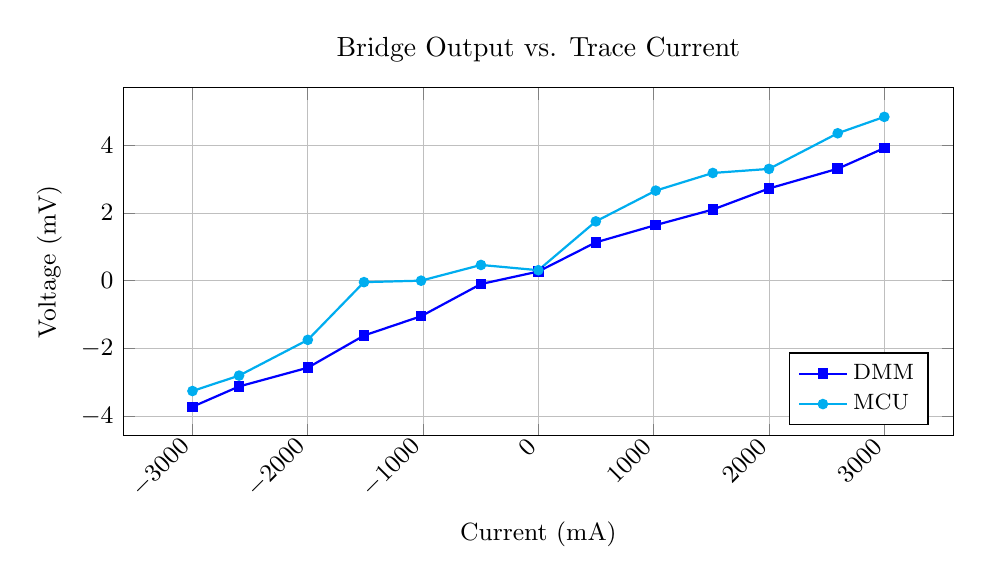
\begin{tikzpicture}
            \begin{axis}[
                width=\textwidth,
                height=6cm, % Squashes vertical height
                title={Bridge Output vs. Trace Current},
                xlabel={Current (mA)},
                ylabel={Voltage (mV)},
                grid=both,
                grid style={line width=.1pt, draw=gray!20},
                major grid style={line width=.2pt, draw=gray!50},
                mark size=1.5pt,
                x tick label style={rotate=45, anchor=east},
                /pgf/number format/1000 sep={},
                label style={font=\small},
                tick label style={font=\small},
                legend pos=south east, % Puts legend in bottom right corner
                legend style={font=\footnotesize, cells={anchor=west}}
            ]
                % First line: DMM Data
                \addplot[color=blue, thick, mark=square*] coordinates {
                    (-2999.0, -3.723) (-2595.0, -3.123) (-1999.0, -2.570)
                    (-1512.0, -1.620) (-1017.0, -1.050) (-498.0, -0.100)
                    (-0.7, 0.269) (498.0, 1.130) (1017.0, 1.640)
                    (1512.0, 2.098) (1999.0, 2.720) (2595.0, 3.303) (2999.0, 3.912)
                };
                \addlegendentry{DMM}

                % Second line: MCU Data
                \addplot[color=cyan, thick, mark=*] coordinates {
                    (-2999.0, -3.258) (-2595.0, -2.803) (-1999.0, -1.748)
                    (-1512.0, -0.044) (-1017.0, -0.001) (-498.0, 0.463)
                    (-0.7, 0.308) (498.0, 1.749) (1017.0, 2.657)
                    (1512.0, 3.178) (1999.0, 3.298) (2595.0, 4.350) (2999.0, 4.834)
                };
                \addlegendentry{MCU}
            \end{axis}
        \end{tikzpicture}
        \captionof{figure}{Plot of irradiated DMM and MCU sweeps detailed in Table~\ref{tab:sensitivity-irr}.}
        \label{fig:sensitivity-irr-dual-plot}
    \end{minipage}
\end{figure}

The same linear-fit procedure gives a sensitivity of \SI{1.269}{\milli\volt\per\ampere} on the DMM ($R^2 = 0.995$) and \SI{1.312}{\milli\volt\per\ampere} on the MCU ($R^2 = 0.975$), corresponding to 93.6\% (DMM) and 99.8\% (MCU) of the unirradiated sensitivity (Section~\ref{sec:sensitivity-fit}). Both figures are well within the level of session-to-session variation already observed on unirradiated hardware (Section~\ref{sec:instr-validation}), with no consistent direction of change between the two independent instruments. \emph{No statistically significant change in sensitivity was found at the tested dose.} Given that this specific radiation configuration does not appear elsewhere in the TMR-sensor literature reviewed for this project (Section~\ref{sec:rad-tolerance-lit}, pending confirmation), this result is offered as a preliminary but novel data point for TMR radiation tolerance under this exposure regime, supporting the broader literature consensus on MTJ radiation tolerance (Section~\ref{sec:rad-tolerance-lit}).

\section{Magnetic Shielding}
\label{sec:shielding}

\subsection{Enclosure Design}
\label{sec:shielding-enclosure}

To address the ambient-field discrepancy identified in Section~\ref{sec:field-discrepancy}, a 3D-printed enclosure incorporating ferrite shielding material was designed. Mu-metal, though offering higher permeability, was not used due to cost constraints; ferrite was selected as a lower-cost alternative offering useful shielding performance. An initial informal test, manually covering and uncovering the sensor with a sheet of nanocrystalline shielding material while monitoring output ripple, showed a clear qualitative reduction in ripple while covered, motivating the purpose-built enclosure. The magnetic shielding progression—including the internal board placement (Figure~\ref{fig:box_pcb}) and the final exterior wrap (Figure~\ref{fig:box_nano})—can be seen in Figure~\ref{fig:shielding_enclosure}.

\begin{figure}[H]
    \centering
    % Define the professional style: Bright cyan lines, clean white badges
    \tikzset{
        badge/.style={fill=white, draw=black!40, thick, rounded corners=2pt, inner sep=3pt, font=\sffamily\small\bfseries, text=black!80},
        pointer/.style={-stealth, draw=cyan, line width=1.5pt}
    }

    % Subfigure A: CAD Model
    \begin{subfigure}[b]{0.32\textwidth}
        \centering
        \begin{tikzpicture}
            \node[anchor=south west, inner sep=0] (imageA) at (0,0) {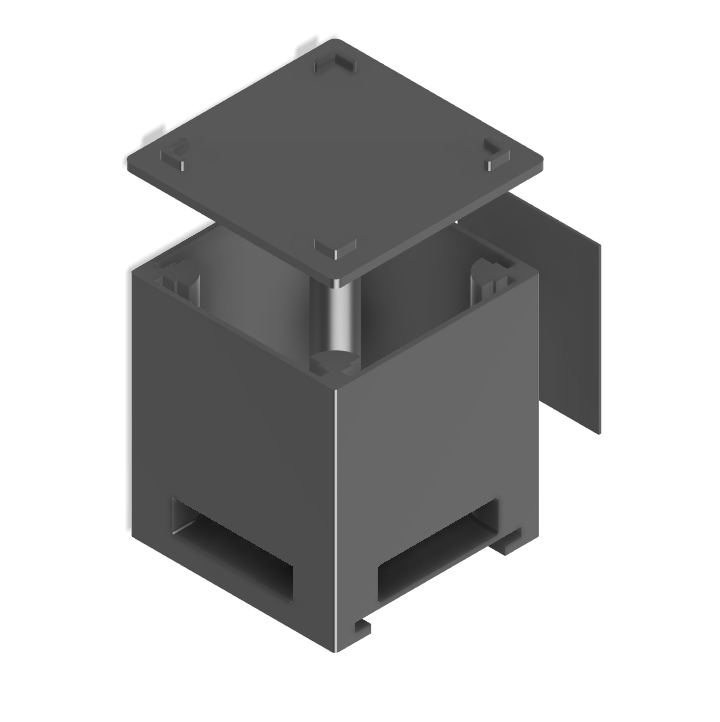
\includegraphics[width=\textwidth]{Box_FINAL_v2 v1.png}};
            \begin{scope}[x={(imageA.south east)},y={(imageA.north west)}]
                % F badge pointing precisely to the bottom right ferrite insertion slot
                \node[badge] (F_cad) at (0.85, 0.1) {F};
                \draw[pointer] (F_cad) -- (0.7, 0.25);
            \end{scope}
        \end{tikzpicture}
        \caption{Enclosure CAD render.}
        \label{fig:box_cad}
    \end{subfigure}
    \hfill
    % Subfigure B: PCB inside the box
    \begin{subfigure}[b]{0.32\textwidth}
        \centering
        \begin{tikzpicture}
            \node[anchor=south west, inner sep=0] (imageB) at (0,0) {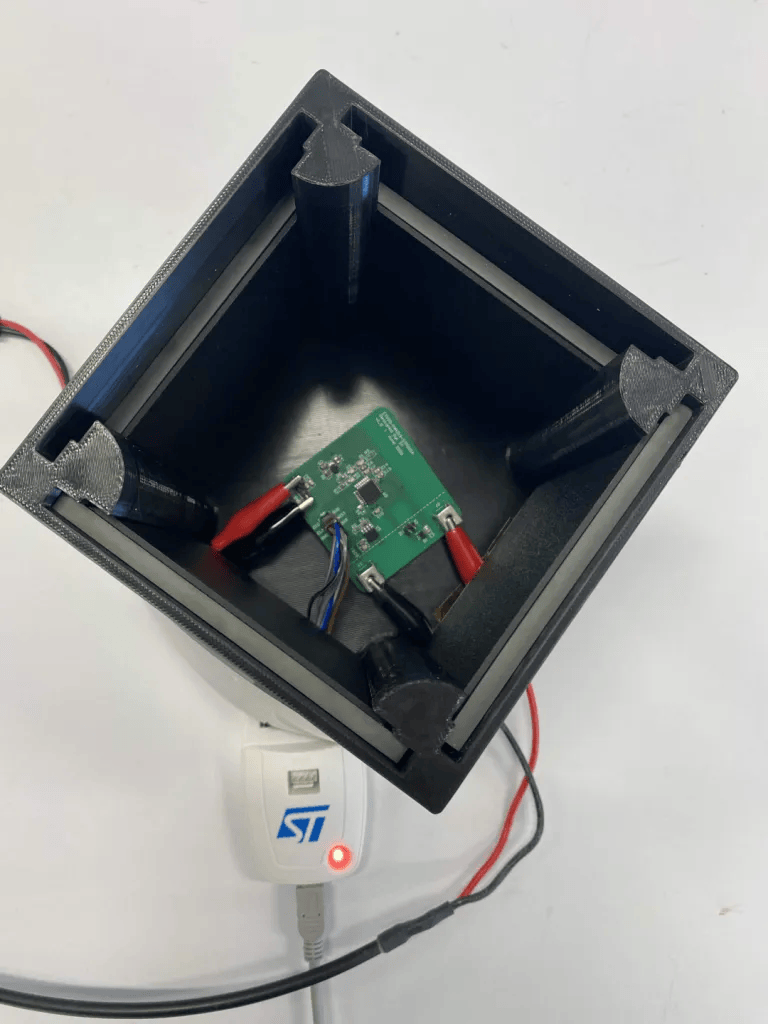
\includegraphics[width=\textwidth]{pcb_box.png}};
            \begin{scope}[x={(imageB.south east)},y={(imageB.north west)}]
                % F badge pointing exactly to the 4 internal ferrite slabs/slots
                \node[badge] (F_pcb) at (0.15, 0.85) {F};
                \draw[pointer] (F_pcb) -- (0.64, 0.73); % Top right slab
                \draw[pointer] (F_pcb) -- (0.80, 0.50); % Bottom right slab
                \draw[pointer] (F_pcb) -- (0.28, 0.40); % Bottom left slab
                \draw[pointer] (F_pcb) -- (0.3, 0.72); % Top left slab
            \end{scope}
        \end{tikzpicture}
        \caption{Internal PCB mounting.}
        \label{fig:box_pcb}
    \end{subfigure}
    \hfill
    % Subfigure C: Fully shielded with Nano/Ferrite layer
    \begin{subfigure}[b]{0.32\textwidth}
        \centering
        \begin{tikzpicture}
            \node[anchor=south west, inner sep=0] (imageC) at (0,0) {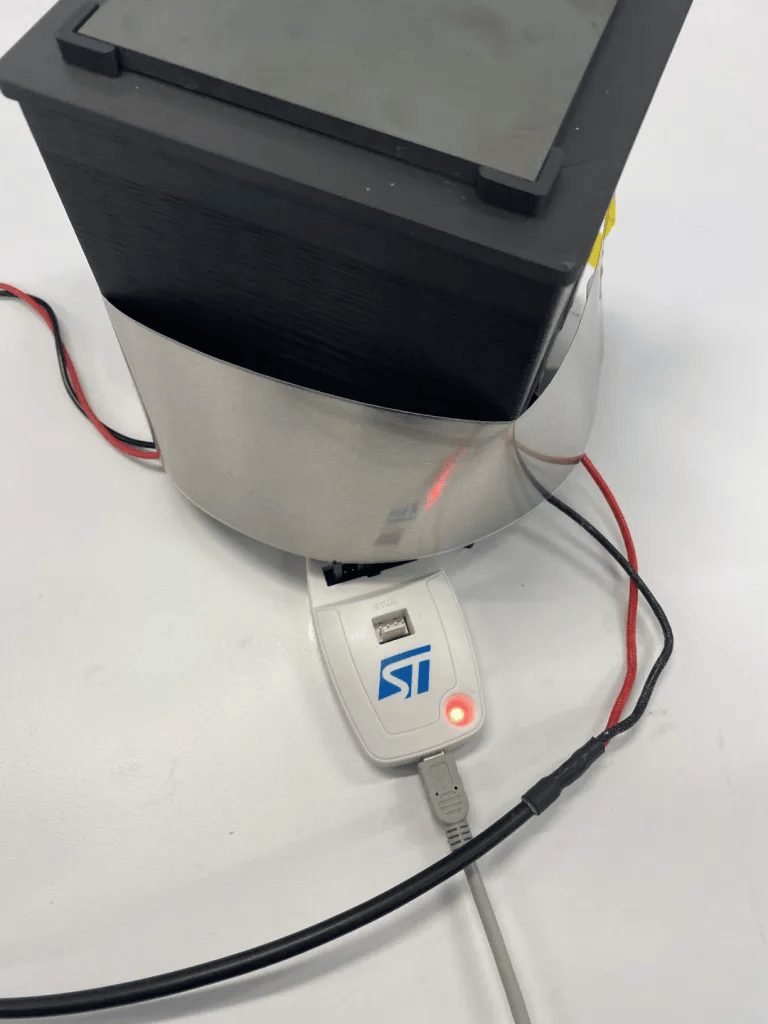
\includegraphics[width=\textwidth]{box_nano.png}};
            \begin{scope}[x={(imageC.south east)},y={(imageC.north west)}]
                % F badge pointing to the top ferrite lid block
                \node[badge] (F_ext) at (0.2, 0.8) {F};
                \draw[pointer] (F_ext) -- (0.55, 0.9);
                
                % N badge pointing directly onto the shiny metal shielding wrap
                \node[badge] (N_ext) at (0.85, 0.2) {N};
                \draw[pointer] (N_ext) -- (0.65, 0.550);
            \end{scope}
        \end{tikzpicture}
        \caption{Exterior shielding layer.}
        \label{fig:box_nano}
    \end{subfigure}
    
    \caption{Development of the magnetic shielding enclosure. (a) The 3D-printed chassis. (b) The integrated sensor board mounted inside. (c) The assembled test configuration wrapped in shielding. Annotations indicate the placement of ferrite plates (\textbf{F}) and flexible nanocrystalline shielding (\textbf{N}).} Maybe say what kinda of ferrite and nano lol
    \label{fig:shielding_enclosure}
\end{figure}
    

\subsection{Shielded Sweep Results}
\label{sec:shielded-results}

With MCU-DMM agreement already established across the full current range (Section~8), the shielded current sweep was conducted using MCU-only logging (no DMM or oscilloscope): the earlier cross-validation (Section~8) showed MCU and DMM readings agreeing to within a fraction of an ADC LSB across the unshielded sweep, so introducing the DMM into the shielded enclosure was judged to add setup complexity and added another source of possible stray magnetic field.

\begin{figure}[H]
    \centering
    
    % Left side: The Table
    \begin{minipage}[c]{0.38\textwidth}
        \centering
        \small
        \captionof{table}{Shielded, non-irradiated current sweep (MCU only): bridge output vs.\ trace current.}
        \label{tab:sensitivity-shielded}
        \begin{tabular}{@{}rr@{}}
            \toprule
            Current (mA) & MCU (mV) \\
            \midrule
            \(-3043.4\) & 8.039 \\
            \(-2522.5\) & 8.549 \\
            \(-2057.7\) & 9.594 \\
            \(-1540.3\) & 9.949 \\
            \(-1040.2\) & 11.170 \\
            \(-546.2\) & 11.319 \\
            \(-6.3\) & 12.705 \\
            $535.4$ & 12.946 \\
            $996.2$ & 13.931 \\
            $1523.0$ & 14.530 \\
            $2038.1$ & 15.532 \\
            $2486.1$ & 16.103 \\
            $2988.7$ & 16.474 \\
            \bottomrule
        \end{tabular}
    \end{minipage}%
    \hfill
    % Right side: The Plot
    \begin{minipage}[c]{0.58\textwidth}
        \centering
        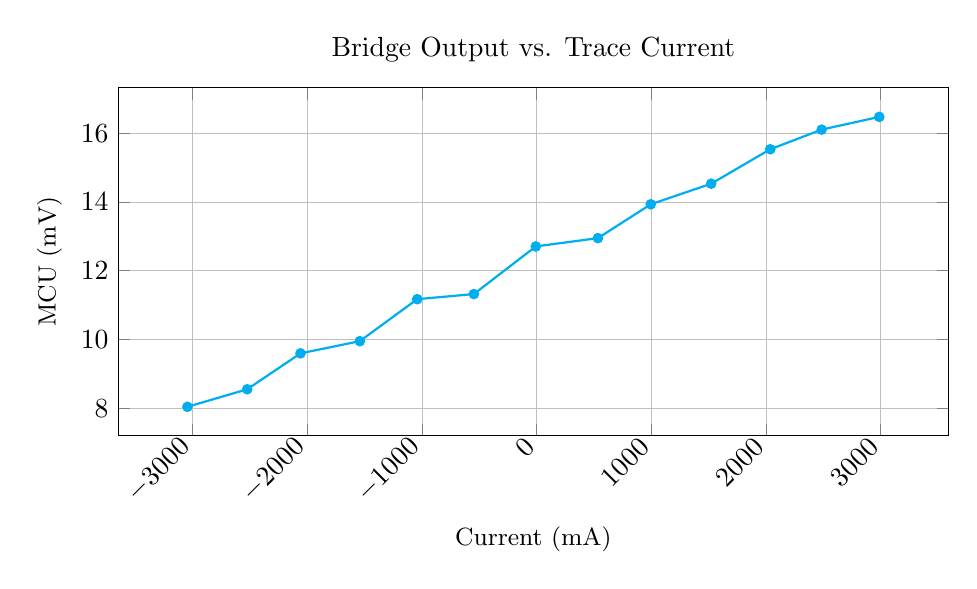
\begin{tikzpicture}
           \begin{axis}[
                width=\textwidth,
                height=6cm,
                title={Bridge Output vs. Trace Current},
                xlabel={Current (mA)},
                ylabel={MCU (mV)},
                grid=both,
                grid style={line width=.1pt, draw=gray!20},
                major grid style={line width=.2pt, draw=gray!50},
                mark size=1.5pt,
                % FIX: Rotate labels and remove the thousands comma
                 label style={font=\small},
                x tick label style={rotate=45, anchor=east},
                /pgf/number format/1000 sep={}
            ]
                \addplot[color=cyan, thick, mark=*] coordinates {
                    (-3043.4, 8.039)
                    (-2522.5, 8.549)
                    (-2057.7, 9.594)
                    (-1540.3, 9.949)
                    (-1040.2, 11.170)
                    (-546.2, 11.319)
                    (-6.3, 12.705)
                    (535.4, 12.946)
                    (996.2, 13.931)
                    (1523.0, 14.530)
                    (2038.1, 15.532)
                    (2486.1, 16.103)
                    (2988.7, 16.474)
                };
            \end{axis}
        \end{tikzpicture}
        \captionof{figure}{Plot of the shielded current sweep data detailed in Table~\ref{tab:sensitivity-shielded}.}
        \label{fig:sensitivity-plot}
    \end{minipage}
\end{figure}

\subsection{Combined Radiation and Shielding Results}

The irradiated integrated board was subsequently tested inside the shielded enclosure (Section~10) under the same sweep procedure, on a sensor that had not previously been driven into saturation.

\begin{figure}[H]
    \centering
    
    % Left side: The Table
    \begin{minipage}[c]{0.38\textwidth}
        \centering
        \small % <--- 1. ADD THIS: Reduces the table text size
        \captionof{table}{Irradiated, shielded current sweep (MCU only): bridge output vs.\ trace current.}
        \label{tab:sensitivity-irr-shielded}
        \begin{tabular}{@{}rr@{}}
            \toprule
            Current (mA) & MCU (mV) \\
            \midrule
            \(-3007.1\) & \(-3.287\) \\
            \(-2501.2\) & \(-2.769\) \\
            \(-2054.6\) & \(-1.130\) \\
            \(-1567.3\) & 0.069 \\
            \(-1037.7\) & \(-0.001\) \\
            \(-532.1\) & 0.107 \\
            \(-6.3\) & 1.318 \\
            $512.5$ & 1.699 \\
            $1011.4$ & 2.837 \\
            $1557.8$ & 3.241 \\
            $2048.6$ & 3.933 \\
            $2560.6$ & 4.807 \\
            $3025.4$ & 4.932 \\
            \bottomrule
        \end{tabular}
    \end{minipage}%
    \hfill
    % Right side: The Plot
    \begin{minipage}[c]{0.58\textwidth}
        \centering
        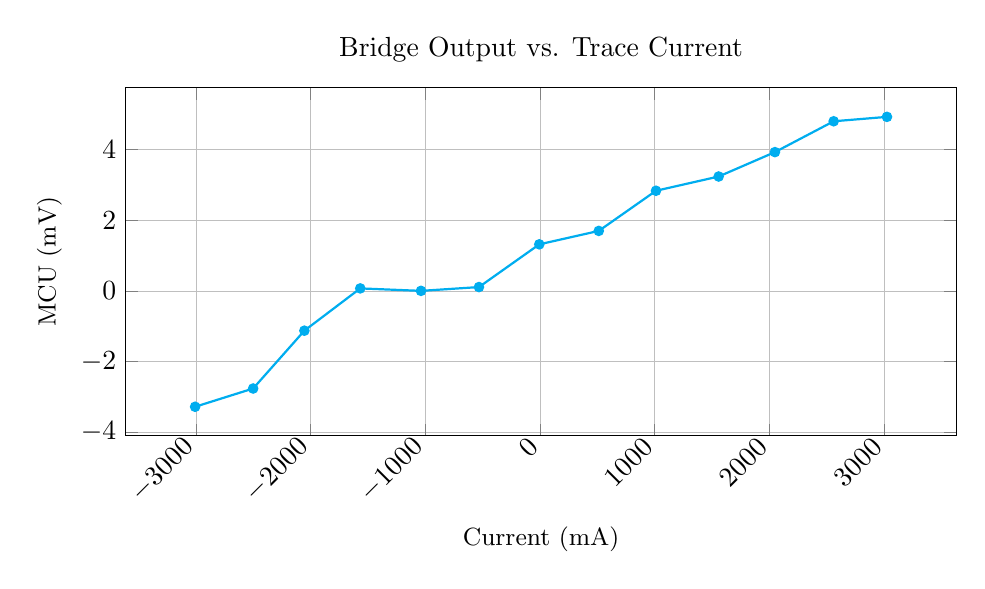
\begin{tikzpicture}
            \begin{axis}[
                width=\textwidth,
                height=6cm,
                title={Bridge Output vs. Trace Current},
                xlabel={Current (mA)},
                ylabel={MCU (mV)},
                grid=both,
                grid style={line width=.1pt, draw=gray!20},
                major grid style={line width=.2pt, draw=gray!50},
                mark size=1.5pt,
                label style={font=\small},
                x tick label style={rotate=45, anchor=east},
                /pgf/number format/1000 sep={}
            ]
                \addplot[color=cyan, thick, mark=*] coordinates {
                    (-3007.1, -3.287)
                    (-2501.2, -2.769)
                    (-2054.6, -1.130)
                    (-1567.3, 0.069)
                    (-1037.7, -0.001)
                    (-532.1, 0.107)
                    (-6.3, 1.318)
                    (512.5, 1.699)
                    (1011.4, 2.837)
                    (1557.8, 3.241)
                    (2048.6, 3.933)
                    (2560.6, 4.807)
                    (3025.4, 4.932)
                };
            \end{axis}
        \end{tikzpicture}
        \captionof{figure}{Plot of the irradiated, shielded current sweep data detailed in Table~\ref{tab:sensitivity-irr-shielded}.}
        \label{fig:sensitivity-irr-plot}
    \end{minipage}
\end{figure}

A linear fit gives a sensitivity of \SI{1.342}{\milli\volt\per\ampere} ($R^2 = 0.975$), corresponding to approximately \SI{3.67}{\milli\volt\per\volt\per\milli\tesla}. This sits close to the unshielded-irradiated result (\SI{1.312}{\milli\volt\per\ampere}, Section~11.4, a 2.3\% difference) and noticeably closer to it than to the unirradiated-shielded result (\SI{1.4465}{\milli\volt\per\ampere}, Section~10.2, a 10\% boost from shielding). In other words, the shielding-driven sensitivity increase clearly observed on the unirradiated board (Section~10.2) was not clearly reproduced on the irradiated board here. \todo{This discrepancy is not yet explained -- possibilities include: the irradiated board's current range and sample spacing differ slightly from the unirradiated sweep (a genuine methodological difference, not yet controlled for); normal session-to-session/board-to-board variation, of the same 3--7\% scale documented throughout this report, happens to have worked in the opposite direction here; or shielding genuinely interacts differently with the irradiated sensor's response. Distinguishing between these needs at least one more shielded-irradiated repeat, ideally in the same session as a shielded-unirradiated control, before drawing a firm conclusion -- do not overstate this in the Discussion/Conclusion beyond \"not yet reproduced\" until that is done.} No statistically significant change in sensitivity attributable to radiation is apparent in either the shielded or unshielded comparison, which remains the primary, better-supported finding of this radiation strand (Section~11.4).

\section{Discussion}
\label{sec:discussion}

The experimental results confirm several of the CT100's key design properties and surface a small number of practical issues to resolve before the hardware can be used as a precision, repeatable test rig.

\textbf{Bridge topology and saturation mechanism.} The $V_{\text{CC}}/3$ saturation ceiling is not merely an empirical observation; Section~\ref{sec:bridge-topology} shows it follows directly from the CT100's specified 20--40~k$\Omega$ per-element resistance range via Equation~\eqref{eq:vsat}, and the measured value (\SI{1.12}{\volt} at $V_{\text{CC}} = \SI{3.30}{\volt}$) matches this derivation closely. This is a useful confirmation: the sensor's saturation ceiling can be predicted from $V_{\text{CC}}$ alone for any future supply condition, without needing to empirically re-characterise it each time.

\textbf{Field-model discrepancy.} The Ansys and analytical models agree closely with each other but under-predict the measured sensor output by roughly a factor of two, and the fitted sensitivity (Section~\ref{sec:sensitivity-fit}) sits about 18\% below the datasheet figure. Because the sensitivity result is a slope and therefore immune to a fixed additive offset, both discrepancies point toward the same explanation: ambient background field pickup in the absence of shielding, rather than an error in the trace model itself. The preliminary shielded results (Section~\ref{sec:shielding-sweep}) moving closer to the simulated prediction support this explanation directly.

\textbf{Saturation recovery and ADCS implications.} The measured \SI{82.3}{\milli\second} recovery time (Section~\ref{sec:sat-recovery-integrated}) is directly relevant to how closely a magnetorquer firing and a magnetometer reading can be scheduled without corrupting the ADCS control loop. \todo{If a specific safe guardband $G$ has been calculated against a target OBC sampling frequency, insert that comparison and result here.}

\textbf{Hysteresis.} The observation that saturation leaves a permanent, linear-but-offset baseline (Section~\ref{sec:standalone-sat-recovery}) is a practically important finding for any CubeSat deployment: it implies the sensor's zero-point cannot be assumed stable across the mission if it experiences even one strong saturating event, and would need either periodic re-calibration or a design that avoids saturating the sensor in the first place. \todo{This finding needs the quantification and reconciliation noted in Section~\ref{sec:standalone-sat-recovery} before it can be stated this firmly.}

\textbf{Radiation tolerance.} The post-irradiation sensitivity sweep (Section~\ref{sec:rad-sweep}) measured 93.6\% (DMM) and 99.8\% (MCU) of the unirradiated sensitivity, with no consistent direction of change between two independent instruments, supporting the literature consensus that MTJ-based TMR sensors tolerate ionising radiation substantially better than conventional CMOS devices. A single irradiated unit, tested once, should still be presented as preliminary evidence; a second, independent irradiated replicate would substantially strengthen this conclusion (Section~\ref{sec:conclusions}).

\begin{figure}[h]
\centering
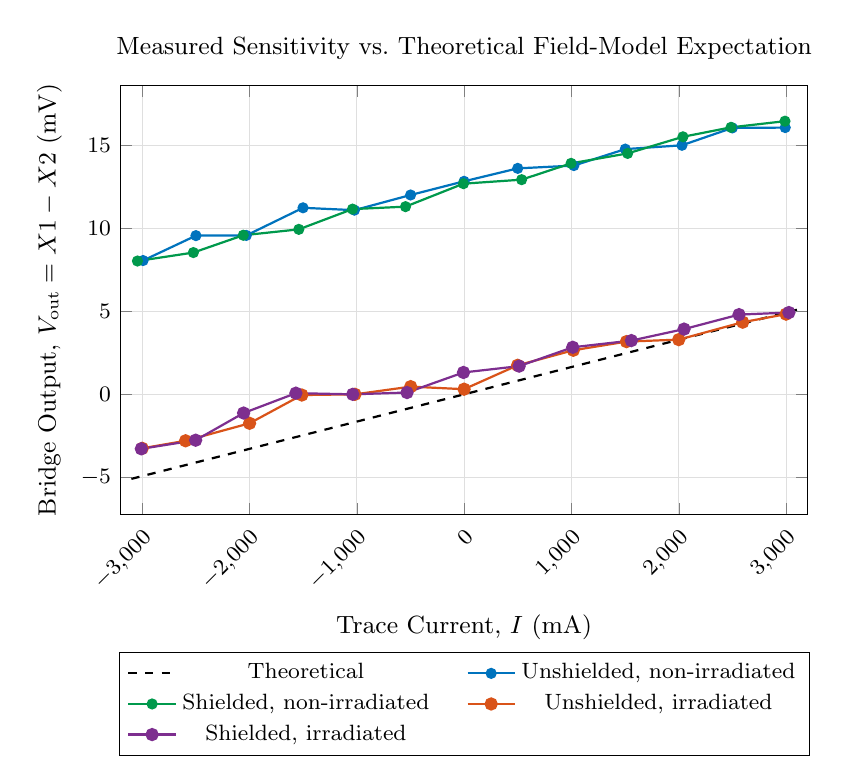
\begin{tikzpicture}
\begin{axis}[
    width=0.85\textwidth,
    height=0.58\textwidth,
    xlabel={Trace Current, $I$ (mA)},
    ylabel={Bridge Output, $V_{\text{out}} = X1 - X2$ (mV)},
    title={Measured Sensitivity vs.\ Theoretical Field-Model Expectation},
    grid=major,
    grid style={gray!25},
    xmin=-3200, xmax=3200,
    axis lines=box,
    tick label style={font=\footnotesize},
    xticklabel style={rotate=45, anchor=north east},
    label style={font=\small},
    title style={font=\small},
    legend columns=2,
    legend style={
        at={(0.5,-0.32)},
        anchor=north,
        font=\footnotesize,
        draw=black,
        /tikz/every even column/.append style={column sep=0.4cm},
    },
]
 
% --- Theoretical / Ansys-model expectation ---
\addplot[black, dashed, thick, domain=-3100:3100, samples=50] {0.0016453*x};
\addlegendentry{Theoretical}
 
% --- Unshielded, non-irradiated ---
\addplot[color={rgb,255:red,0;green,115;blue,189}, mark=*, mark size=1.6pt, thick]
    coordinates {
    (-2991.0,8.069) (-2498.5,9.571) (-2029.0,9.584) (-1501.0,11.249)
    (-1022.0,11.107) (-499.0,12.022) (-0.7,12.847) (499.0,13.628)
    (1022.0,13.796) (1501.0,14.790) (2029.0,15.020) (2498.5,16.068)
    (2991.0,16.088)
    };
\addlegendentry{Unshielded, non-irradiated}
 
% --- Shielded, non-irradiated ---
\addplot[color={rgb,255:red,0;green,153;blue,76}, mark=*, mark size=1.6pt, thick]
    coordinates {
    (-3043.4,8.039) (-2522.5,8.549) (-2057.7,9.594) (-1540.3,9.949)
    (-1040.2,11.170) (-546.2,11.319) (-6.3,12.705) (535.4,12.946)
    (996.2,13.931) (1523.0,14.530) (2038.1,15.532) (2486.1,16.103)
    (2988.7,16.474)
    };
\addlegendentry{Shielded, non-irradiated}
 
% --- Unshielded, irradiated ---
\addplot[color={rgb,255:red,217;green,83;blue,25}, mark=*, mark size=2pt, thick]
    coordinates {
    (-2999.0,-3.258) (-2595.0,-2.803) (-1999.0,-1.748) (-1512.0,-0.044)
    (-1017.0,-0.001) (-498.0,0.463) (-0.7,0.308) (498.0,1.749)
    (1017.0,2.657) (1512.0,3.178) (1999.0,3.298) (2595.0,4.350)
    (2999.0,4.834)
    };
\addlegendentry{Unshielded, irradiated}
 
% --- Shielded, irradiated ---
\addplot[color={rgb,255:red,125;green,46;blue,143}, mark=*, mark size=2pt, thick]
    coordinates {
    (-3007.1,-3.287) (-2501.2,-2.769) (-2054.6,-1.130) (-1567.3,0.069)
    (-1037.7,-0.001) (-532.1,0.107) (-6.3,1.318) (512.5,1.699)
    (1011.4,2.837) (1557.8,3.241) (2048.6,3.933) (2560.6,4.807)
    (3025.4,4.932)
    };
\addlegendentry{Shielded, irradiated}


\end{axis}
\end{tikzpicture}
\caption{Measured bridge output vs.\ trace current across all four test conditions, against the theoretical field-model expectation (CT100 datasheet sensitivity of \SI{4.5}{\milli\volt\per\volt\per\milli\tesla}). All four measured conditions fall below the theoretical line, consistent with the ambient-field-driven discrepancy discussed in this section; the shielded, non-irradiated condition sits closest to it. Note each dataset carries its own session-specific baseline offset here; see Figure~\ref{fig:sensitivity-comparison} for a baseline-corrected, slope-only comparison.}
\label{fig:sensitivity-comparison-raw}
\end{figure}

\textbf{Limitations.} The hand-held Neodymium magnet used to drive saturation in Section~\ref{sec:sat-test-methodology} is not a repeatable or automatable stimulus (Section~\ref{sec:conclusions}). The irradiated sample underwent an additional desolder/resolder thermal cycle during transfer to its readout board, which the unirradiated reference sensor did not undergo; a dedicated process control was not performed given time constraints, so a small contribution from thermal rework to the observed pre/post-irradiation difference cannot be fully excluded.

\section{Conclusions and Future Work}
\label{sec:conclusions}

\textbf{Key findings.}
\begin{itemize}
\item The CT100's $V_{\text{CC}}/3$ saturation ceiling is derived directly from its specified per-element resistance range (20--40~k$\Omega$) and confirmed experimentally (\SI{1.12}{\volt} measured at $V_{\text{CC}} = \SI{3.30}{\volt}$).
\item Saturation leaves the sensor at a new, offset-but-linear baseline rather than the original zero-field value, a hysteresis effect with direct implications for in-mission recalibration. \todo{Pending quantification -- see Section~\ref{sec:standalone-sat-recovery}.}
\item Measured sensitivity is \SI{3.7}{\milli\volt\per\volt\per\milli\tesla}, approximately 18\% below the CT100's \SI{4.5}{\milli\volt\per\volt\per\milli\tesla} datasheet figure, most plausibly attributable to ambient-field pickup in the absence of shielding rather than a sensor shortfall.
\item Saturation recovery on the integrated board takes \SI{82.3}{\milli\second} ($\approx \SI{12.15}{\hertz}$), directly relevant to ADCS guardband design around magnetorquer firings.
\item Radiation testing found no statistically significant change in sensitivity pre- vs.\ post-irradiation (93.6--99.8\% of the unirradiated value), a preliminary but potentially novel data point for this specific exposure regime.
\item An initial shielded enclosure showed a qualitative improvement toward simulated field predictions, supporting ambient pickup as the cause of the field-model discrepancy above.
\end{itemize}

\textbf{Future work.}
\begin{itemize}
\item \textbf{Improve the saturation stimulus.} The hand-held magnet is acknowledged as a limiting factor throughout this report. Given that radiation has now been shown to have no significant effect on sensitivity, remaining time is better spent developing a more repeatable, automated saturation source (e.g.\ a driven electromagnet or Maxwell coil) and re-running the full characterisation on the non-irradiated integrated board, rather than further radiation testing.
\item Complete and quantify the shielded and radiation-plus-shielded sweeps (Sections~\ref{sec:shielding-sweep} and \ref{sec:combined-rad-shielding}).
\item Quantify the hysteresis offset magnitude and confirm its stability over repeated saturation cycles.
\item Repeat the saturation-recovery measurement multiple times to report a mean $\pm$ standard deviation rather than a single trial, and add a hysteresis (up/down current sweep) linearity measurement.
\item Obtain a second, independent irradiated replicate, ideally on an unreworked board, to strengthen the single-unit radiation-tolerance conclusion and control for the resolder-cycle limitation noted in Section~\ref{sec:discussion}.
\item Implement the non-zero reference-bias design change proposed in Section~\ref{sec:future-pcb-note} on a future PCB revision.
\end{itemize}

\textbf{Overall conclusion.} Based on the evidence gathered to date, the CT100 TMR sensor appears viable for CubeSat ADCS/EPS applications: its bridge behaviour is well-characterised and predictable, its sensitivity is within a reasonable margin of its datasheet specification once ambient-field effects are accounted for, and it shows no measurable radiation-tolerance penalty at the dose tested. This should be read as an encouraging preliminary result rather than a qualification conclusion; the future work above, particularly a repeatable saturation source and a second irradiated replicate, would be needed to state this with confidence.

% ============================================================
% PAGE-COUNT RANGE END (Introduction -- Conclusions)
% ============================================================


\begin{thebibliography}{99}

 \bibitem{ct100_datasheet}
Allegro MicroSystems, \emph{CT100 1D Linear TMR Sensor Datasheet}, CT100-DS Rev. 3, 2023.

\bibitem{survey-magnetic-sensing} ``A Survey on Magnetic Sensing and Communication: Technologies, Sensors, and Applications,'' \emph{IEEE Journals \& Magazine}, IEEE Xplore.

\bibitem{amr-gmr-hall-bridging} ``Bridging The Gap Between AMR, GMR, And Hall Magnetic Sensors,'' \emph{IEEE Conference Publication}, IEEE Xplore.

\bibitem{magic-radcube} ``In Flight Performance of the MAGIC Magnetoresistive Magnetometer on the RadCube CubeSat,'' \emph{Space Science Reviews} (Springer).

\bibitem{alves-thesis} P.\ F.\ L.\ Alves, ``Radiation Hardness Assessment of MR sensors for Space Applications,'' MSc thesis, available via lip.pt.

\bibitem{tmr-bias-radiation} ``Radiation tolerance of tunneling magnetoresistance sensors under bias voltage,'' \emph{Science China / Springer}.

\bibitem{tid-basics-lanl} ``Basic Mechanisms: Total Ionizing Dose,'' Los Alamos National Laboratory presentation.

\end{thebibliography}

\end{document}